\scanpage{3}
\uline{N° 1} Notions sur les réarrangements de fonctions

\uline{N° 2} \unsure{Fonctions} de Weyl.

\uline{N° 3} Inégalités \deleted{de \unsure{convexité liées aux réarrangements}}\inserted{\unsure{fondamentales}}
\((A\in\bar a)\)

\uline{N° 4} Mesures \unsure{spectrales}, réarrangement \deleted{\unsure{spectral}}\inserted{\unsure{décroissant}} d'un opérateur. \((A\in\widetilde{\bar a})\)

\deleted{\unsure{Premières propriétés des valeurs propres} \deleted{\unsure{sp.|de}} \unsure{d'un} \unsure{A}}

\deleted{\unsure{N° 5}}
\uline{N° \unsure{5|6}} Compléments sur le déterminant

\uline{N° 6} L'\deleted{\unsure{a}}inégalité \deleted{de convexité dans les espaces d'\unsure{opérateurs}}\inserted{\unsure{fondamentale} \deleted{\unsure{pour}} \(AB\)}

\uline{N° 7} Autres inégalités.

\mspage{2}

\scanpage{4}
Soit \(C\) une \(C^*\)-Algèbre, on veut déterminer les \deleted{\unsure{endomorphismes}} endomorphismes linéaires continus \(T\) permutant aux translations gauches. Soit \(T\) un tel, on \unsure{notera|voit} que \(T''\) est un endomorphisme \unsure{fblt} continu \inserted{de \(C''\)} qui permute aux translations \(x\to xy\) \deleted{\((y\in C)\) \unsure{donc}} pour \(y\in C\), donc pour \(\forall y\in C''\) \inserted{donc} \(\bigl(T''(xy)=T''(x)y\quad\deleted{\unsure{il est même déjà}}\inserted{les deux}\text{ mbs sont \unsure{fblt} continus}\bigr)\).

Donc de la forme \(x\to ax\) \((a\in C'')\)\inserted{\unsure{bien déterminé car} \(a=\unsure{T''(1)}\)}, En fait, \(a\) appartient à l'ens.\inserted{\(\Gamma_g\)} des éléments \(a\) de \(C''\) tels que \(aC\subset C\). On voit donc que l'ensemble d'endomorphismes considéré est isomorphe, avec sa structure d'algèbre normée, à \(\Gamma_g\), \deleted{\unsure{T herm.}} \(a\) hermitien signifie \(x^*T(x)\) hermitien pour tout \(x\in C\); \(a\) positif signifie \(x^*T(x)\geq0\) pour \deleted{tout} \(x\in C\).

Soit \deleted{\unsure{g}} \(\Gamma\) l'ens des \(a\in C''\) tels que \(a\uline{C}\subset\uline{C},\ \uline{C}a\subset\uline{C}\). C'est une sous. \(C^*\)-Algèbre involutive. \unsure{T. él\textsuperscript{t}|Tout élément} hermitien de \(\Gamma_g\) est dans \(\Gamma\).

Supposons maintenant \(C\) plongé dans la \(C^*\)-Algèbre \(R\), et soit \(\Gamma_1\) l'ens des \(x\in R\) tels que \(xC\subset C,\ \unsure{Ca|Cx}\subset R\), c'est une sous \(C^*\)-algèbre de \(R\). Pour tout \(a\in\Gamma_1\), soit \(\varphi(a)\) l'élément de \(C''\) correspondant : l'opération \(T_a x=ax\) dans \(C\). Si \(a\) hermitien, \(\varphi(a)\) est hermitien, donc dans \(\Gamma\), donc pour \(\forall a\in\Gamma_1\), \(\varphi(a)\in\Gamma\); De plus, \(\varphi\) est évidemment une représentation d'algèbre, compatible avec l'involution (\unsure{puisque}

\mspage{5}

\scanpage{5}
\unsure{transforme} hermitiens en hermitiens). On a en \unsure{particulier} un \uline{accouplement} entre \(\Gamma\) et \(C'\), positif etc. On a
\[
\varphi(a)=\lim_{\substack{\deleted{\unsure{x\in C}}\\\deleted{\unsure{1\,\mathrm{fbt}}}\;\inserted{x\xrightarrow{\unsure{\mathrm{fbt}}}1}\\\unsure{\wedge}\\C}}ax
=\lim_{\substack{x\to1\\\unsure{\wedge}\,\unsure{\mathrm{fbt}}\\C}}xa,
\]
(\unsure{limite faible} dans \(C''\)), d'où \deleted{\unsure{g}}
\[
\langle a,f\rangle=\lim_{\substack{x\to1\\\unsure{\wedge}\,\unsure{\mathrm{fbt}}\\C}}\langle ax,f\rangle
\]
\((a\in\Gamma_1,\ f\in C')\), et cet accouplement est compatible avec ordre, involution etc, et prolonge celui donné sur \(C\times C'\).

Supposons maintenant que \(R\) est un anneau de von Neumann,\inserted{et \(C\) dense dans \(R\)} d'où \unsure{canonique} \(\psi:C''\to R\) (\unsure{applique} \(C''\) sur l'adhérence faible de \(C\) dans \(R\)). Évidemment \(\psi(\Gamma)\subset\Gamma_1\). D'autre part,
\[
\varphi\psi\deleted{\unsure{(u)}}=1\quad\text{sur }\Gamma,
\]
car soit \(u\in\Gamma\), \deleted{\illegible{1}} et \(\unsure{v}=\psi(u)\in\Gamma_1\), on a pour \(\forall f\in R_*\)
\[
\langle v,f\rangle=\langle u,f_1\rangle
\]
\((f_1\text{ image de }f\text{ dans }C';\;\text{en fait on a une injection }R_*\subset C')\).
J'affirme que
\[
\langle v,f\rangle=\langle\varphi(\unsure{v}),f_1\rangle
\]
[ce qui prouve \deleted{que} \(\varphi(\unsure{v})\unsure{-}u\) orthogonal à \(R_*\)] cela se voit facilement car
\[
\langle\varphi(\unsure{v}),f_1\rangle=\lim_{x\to1}\langle vx,f\rangle
\]
en prenant ici le filtre des sections \unsure{croissantes des éléments} \(x\unsure{\ll}1\) de \(C\). \unsure{On est ramené} à prouver : un élément de \(\uline{\Gamma}\) orthogonal à \(R_*\) \deleted{\unsure{est nul}} (i.e. dont l'image dans \(R\) est \(0\)) est nul. C'est immédiat

\mspage{6}

\scanpage{6}
car si \(x\) est un tel \unsure{élém.}, alors pour \(y\in C\) on a
\[
\unsure{\psi|\varphi}(xy)=\unsure{\psi|\varphi}(x)y=0,
\]
d'où (comme \(xy\in C\), \unsure{alors|déjà} \(\unsure{\psi|\varphi}(xy)=xy\)) \(xy=0\), et ceci pour tout \(y\in C\), d'où \(x=0\). -- \uline{Donc \(\psi\) est un isomorphisme de \(\Gamma\) sur \(\Gamma_1\)}, \deleted{(\unsure{et le} \(\varphi\) \unsure{est la réciproque})}\inserted{\deleted{\unsure{et}} dont \(\varphi\)} \uline{est l'inverse}.

\unsure{Il n'y a plus} qu'à prouver que \(\psi\varphi=1\), soit donc \(u\in\Gamma_1\)
\[
\varphi u=v\in C''\quad\text{est donné par}\quad\langle v,f\rangle=\uline{\langle u,f\rangle}\quad(f\in C')
\]
\deleted{\unsure{d'où|alors}} \(\psi v\) est donné par
\[
\langle\psi v,f\rangle=\langle v,f_1\rangle\quad(f\in R_*)
\]
i.e.
\[
\langle\psi v,f\rangle=\langle u,f_1\rangle\quad(f\in R_*),
\]
mais on a déjà dit que \(\langle u,f_1\rangle=\langle u,f\rangle\), d'où
\[
\langle\psi v,f\rangle=\langle u,f\rangle,\quad\text{i.e. }\psi v=u.\qquad\text{CQFD.}
\]

\mspage{7}

\scanpage{7}
Mesures spectrales et réarrangements de fonctions.

\margin{\(\unsure{l}(M),\ L^1(M),\ L^\infty(M)\)\par \(K(M)\)\par \(\unsure{K^\infty(M)|K^\alpha(M)}\)\par \(C_0(M)\)\par \deleted{\(\unsure{\Phi|R}\)}}

Soit \(f\) une fonction mesurable complexe sur l'espace mesuré \(M\) (muni de la mesure \(m\)). On dit que \(f\) \uline{admet une mesure spectrale} si l'image de \(m\) par \(f\) en tant que mesure sur \(\underline C^*\) existe. Cela signifie donc aussi que pour \(0<a<b<+\infty\), \(|f|^{-1}([a,b])\) est intégrable (donc cette condition ne dépend que de \(|f|\)). \(f(m)\) (considérée comme mesure sur \(C^*\)) est appelée \uline{mesure spectrale de \(f\)}, et notée \(\mu_f\) :
\[
(1)\qquad \mu_f=f(m)\qquad\text{i.e.}
\]
\[
(2)\qquad\langle\alpha,\mu_f\rangle=\langle\alpha\circ f,m\rangle=\int\alpha\circ f\,dm
\qquad\deleted{\unsure{\alpha\circ f\,dm}}
\]
pour toute fonction continue à support \unsure{compact} sur \(\underline C^*\). \(\mu_f\) est \uline{positive}. Elle est portée par \(\underline R_*\) (resp. par \(R_*^+\)) \uline{si et seulement si \(f\) est réelle} (resp. positive). \deleted{\unsure{Deux}} Une fonction \(f\) sur l'espace mesuré \(M\) et une fonction \(g\) sur l'espace mesuré \(N\) sont dites \uline{spectralement équivalentes} si elles admettent une même mesure spectrale.

\uuline{Exemples} Si l'ensemble \(f^{-1}(\unsure{\{\ne0\}|\complement\{0\}})\) est intégrable, alors \(\mu_f\) existe et est bornée. C'est en particulier le cas si \(f\) est à support compact, ou si \(m\) est bornée.
\inserted{\unsure{Autre cas : toute} \(f\in C_0(M)\), \unsure{plus généralement telle} que, \deleted{\(\unsure{\varepsilon}\)} pour tout \(\varepsilon\), \(|f|^{-1}(]\varepsilon,\infty[)\) est intégrable.}

\margin{\unsure{continuité}\par\unsure{à gauche}}
\uline{Proposition 1} \deleted{\(\unsure{0}\)} Une fonction positive décroissante \(\varphi\) sur \(R_*^+\) \(\bigl[\) a une mesure spectrale si et seulement si elle est nulle à l'infini; \(\mu_\varphi\) est une mesure positive sur \(R_*^+\) telle que
\[
\int_1^\infty d\mu_\varphi<+\infty.
\]
Réciproquement, pour toute mesure positive \(\nu\) sur \(R_*^+\) telle que \(\int_1^\infty d\nu<+\infty\), existe une fonction \inserted{positive} décroissante \(\varphi\) et une seule (à une \uline{modification} \deleted{\unsure{sur un ensemble}}\inserted{négligeable} près) \unsure{qui admette} \(\nu\) comme mesure spectrale.

On a donc pour presque tout \(t\)
\[
(3)\qquad t=\int_s^\infty d\unsure{\mu|\nu}(s)\qquad(\text{si }s=\varphi(t))
\]

\mspage{8}

\scanpage{8}
les \(t\) exceptionnels étant ceux pour lesquels le second membre de \((\unsure{1|3})\) est ambigu, i.e. qui ne sont pas de mesure nulle pour \(\unsure{\nu|t}\). Ainsi \(\varphi\) apparaît simplement comme fonction inverse de
\[
s\to\int_s^\infty d\unsure{\nu}(s).
\]

\deleted{\uuline{Définition}}
\uline{Corollaire} Soit \(f\) une fonction mesurable positive sur l'espace mesuré \(M\). Pour que \(f\) soit spectralement équivalente à une fonction décroissante \(\varphi\) sur \(R_*^+\), il faut et il suffit que pour tout \(a>0\), \(f^{-1}([a,+\infty[)\) soit intégrable. Alors \(\varphi_{\deleted{\unsure{f}}}\) est \unsure{unique|uniquement} \unsure{déterminée|déterminé}.

\deleted{\unsure{Définition}} On l'appelle le \uline{réarrangement décroissant} de \(f\), noté \(\varphi_f\). Si \deleted{\(\unsure{f_*}\)} \(g\) est une autre fonction mesurable positive, sur un espace mesuré \(N\), satisfaisant aux conditions ci-dessus, alors \(f\) et \(g\) sont \deleted{\unsure{spectralement}} équivalentes si et seulement si elles ont même réarrangement décroissant.
\deleted{\unsure{Si} \(\unsure{E}\) \unsure{est un} \illegible{3}}\inserted{\(\varphi_f(t)\) est défini par}
\[
(4)\qquad
\varphi_f^-(t)=\inf_{\substack{E\subset M\\m(E)\unsure{<|\leq}t}}\|(1-E)f\|_\infty
\qquad
\varphi_f^+(t)=\inf_{\substack{E\subset M\\m(E)\leq t}}\|(1-E)f\|_\infty
\]
où \deleted{\(\unsure{\varphi_f(t)}\)} on pose
\[
\varphi^-(t)=\lim_{\substack{s\to t\\s<t}}\varphi(s),
\qquad\deleted{\unsure{\text{continuité à droite}}}\inserted{\varphi_f^+(t)=\lim_{\substack{s\to t\\s>t}}\varphi(s)}.
\]
\inserted{\unsure{Ainsi on identifie}} un ensemble mesurable \(E\) avec sa fonction caractéristique, ce qui donne un sens à (4). De (4) on tire les formules (pour des fonctions mesurables positives sur un même espace mesuré \(M\)) \deleted{\unsure{f et g étant} \illegible{5}} :
\[
(5)\qquad
\left\{\begin{aligned}
\varphi_f&\leq\varphi_g\quad\deleted{\unsure{\text{implique}}}\inserted{\text{si}}\quad\deleted{\unsure{\varphi_f\leq\varphi_g}}\quad f\leq g\\
\varphi_{\lambda f}&=\lambda\varphi_f\qquad\text{si }\lambda\geq0\\
\varphi_{f^\alpha}&=(\varphi_f)^\alpha\qquad\text{si }\alpha\unsure{>|\geq}0\\
\varphi_{f+g}&\leq\varphi_f+\varphi_g\\
\varphi_{fg}&\leq\varphi_f\varphi_g
\end{aligned}\right.
\]
\margin{\(\int f\,dm=\int s\,d\mu_f(s)\) d'où\par \(\int f\,dm=\int\varphi_f\,dt\)\par\(\unsure{N_p}(f)=\unsure{N_p}(\varphi_f)\) etc.}
\margin{plus généralement pour toute fonction \deleted{\unsure{monotone}}\inserted{\unsure{croissante}} \(\alpha\) sur \(R^+\), \deleted{\unsure{existe}}\par\(\varphi_{\alpha(f)}=\alpha(\varphi_f).\quad\Leftarrow\)\par\deleted{\unsure{positive dans le cas} \(f\) \illegible{4} \(\unsure{g=|f|}\)}\par\deleted{\(\varphi_{|f|}=|\varphi_f|\) \unsure{etc}}}

\deleted{Dans la première formule}, (si \(\varphi_g\) existe \deleted{\(\unsure{\varphi}\)}\inserted{et \(f\leq g,\ \varphi_f\)} existe aussi; si \(\varphi_f\) et \(\varphi_g\) existent, \inserted{\(\unsure{\varphi_{\alpha(f)}}\),}\(\varphi_{f+g}\) et \(\varphi_{fg}\) existent).

Soit \(\psi\) une fonction décroissante sur \(R_*^+\), admettant la mesure spectrale \(\unsure{\mu_\psi}\). Pour que

\mspage{9}

\scanpage{9}
\(\unsure{\varphi|\psi}\) soit sommable au voisinage de \(0\), on voit aussitôt qu'il faut et suffit que
\[
\int_1^\infty d\sigma\int_\sigma^\infty d\mu(s)<+\infty,
\qquad\text{i.e.}\quad\int_1^\infty(s-1)d\mu(s)<+\infty,
\]
\unsure{ce qui signifie} que
\[
\boxed{(6)\quad\int_1^\infty s\,d\mu(s)<\deleted{\unsure{\text{soit}}}+\infty}
\]
\deleted{\unsure{condition. Si} \(\mu=\mu_f\) (\(f\) fonction mesurable sur l'espace mesuré \(M\))}\inserted{Ceci est vérifié quand \(\unsure{\nu|f}\) est bornée, p.ex.} quand \(\nu=\mu_f\), \(f\) étant \unsure{comme dans les exemples, ou bornée}.

\deleted{Si alors \(\unsure{\mu_f}\) satisfait à \(\unsure{(6)}\)}
Si \(\varphi_f\) est sommable au voisinage de \(0\), on pose
\[
(7)\qquad\Phi_f(t)=\int_0^t\varphi_f(s)\,ds
\]
\(\Phi_f(t)\) est une fonction continue concave croissante de \(t\).
\inserted{\unsure{Considérons|En considérant} \(\log\unsure{\varphi_f(t)|\Phi_f(t)}\), c'est une fonction \deleted{décroissante}\inserted{\unsure{concave}}, à valeurs dans \([-\infty,+\infty[\).}
Enfin, supposons \(\log\varphi_f(t)\) sommable au voisinage de \(+0\) (\unsure{a fortiori} \(\varphi_f\) le soit),\inserted{i.e. \(\log f\) sommable dans \(f^{-1}([1,+\infty[)\)} \deleted{\(\log\varphi_f(t)\) \unsure{est}} Nous posons alors
\[
(8)\qquad\Psi_f(t)\unsure{=}\int_0^t\log\varphi_f(\unsure{t|s})
\]
Si \(\varphi_f\) ne s'annule pas \deleted{\unsure{limite à} \(\unsure{+\infty}\) \illegible{2}} (i.e. si \(f^{-1}(\unsure{\complement\{0\}})\) n'est pas \uline{intégrable}) \(\Psi_f(t)\) est une fonction partout finie. Sinon, si \(t_0=|f^{-1}(\complement\{0\})|\) est le \(t\) à partir duquel \(\varphi_f\) est nulle, c'est le point à partir duquel \(\Psi_f(t)\) est égale à \(-\infty\).

Enfin, on pose
\[
(9)\qquad\Delta_f(t)=\exp\Psi_f(t)
\]
Sous les conditions envisagées sur \(f\), \(\Delta_f(t)\) est une fonction continue \deleted{positive}\inserted{\unsure{convexe|concave}} de \(t\); elle ne peut s'annuler que si \(t_0=|f^{-1}(\complement\{0\})|\) est fini, alors \(\Delta_f(t)\) s'annule constamment à partir de \(t_0\).

Les formules (5) donnent des inégalités correspondantes pour \(\Phi_f,\ \Psi_f,\ \Delta_f\). La plus importante est
\[
(10)\qquad\Psi_{fg}\leq\Psi_f+\Psi_g\qquad\text{i.e.}
\]
\[
(11)\qquad\Delta_{fg}\leq\Delta_f\Delta_g
\]

\mspage{10}

\scanpage{10}
\deleted{Supposons \unsure{maintenant que} \(\varphi_f\) \illegible{1}}

On posera, pour une fonction mesurable \deleted{positive}
\[
(12)\qquad\Delta(f)=\Delta^{\unsure{-}}_{|f|}(|M|)=\uuline{\exp}\int_M\log|f|\,dm
\]
\deleted{\(\Delta\) existe \unsure{si}}\par\deleted{donc}
\(\Delta(f)\) existe \deleted{\(\unsure{\Psi_f}\) \unsure{existe}} si \(\log|f|\) est sommable sur l'ens des points où elle est positive. \(0\leq\Delta(f)<+\infty\).
\(\Delta\) jouit des propriétés d'un \inserted{module de} déterminant, en particulier
\[
(13)\qquad\Delta(fg)=\Delta(f)\Delta(g)\qquad\Delta(1)=1
\]
\figure{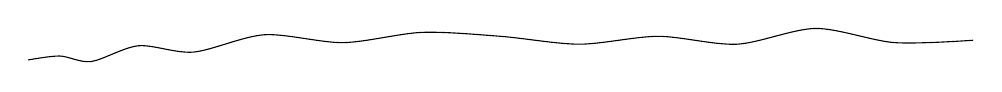
\begin{tikzpicture}[x=1cm,y=1cm]
\draw plot[smooth] coordinates {(0,0) (.4,.05) (.8,-.02) (1.4,.18) (2.1,.1) (3,.32) (4,.22) (5,.35) (6,.3) (7,.2) (8,.3) (9,.2) (10,.4) (11,.22) (12,.25)};
\end{tikzpicture}}

Supposons que \(|M|<+\infty\). On vérifie aussitôt que \deleted{\unsure{si} \(f\)}\inserted{pour une fonction mesurable positive sur \(M\), on a} \deleted{\unsure{étant son} réarrangement décroissant \(\varphi_f\), alors}\par\deleted{il en est de même}\par\deleted{\(\unsure{\varphi_{1+f}}\) \unsure{et}}
\[
(14)\qquad\varphi^-_{\unsure{\lambda|1}+f}(t)\unsure{=|\equiv}\unsure{\lambda|1}+\varphi_f^-(t)\qquad\text{si }\unsure{0<t|0\leq t}\leq|M|
\]
(si \(\varphi_f\) existe; si même \(|M|=\infty\), \(\varphi_{1+f}\) n'existe pas \inserted{\unsure{à priori}} si \(f\geq0\), \deleted{Cependant}\inserted{nous} \unsure{pouvons encore le définir} par (14). Alors \(\log\varphi_{1+f}(t)=\log(1+\varphi_f)\)\deleted{\unsure{si} \(\Phi_f\) existe, \unsure{alors}}\inserted{\(\log(1+\varphi_f)\)} qui est une fonction positive. Si on suppose que \(\Phi_f\) existe, alors \(\log(1+\varphi_f)\) est sommable au voisinage de \(0\) (et dans ce cas seulement). On pose, par définition
\[
(15)\qquad\Delta_{\unsure{\lambda|1}+f}(t)=\exp\int_0^t\log|1+\varphi_f(\unsure{s|u})|\,ds
\qquad0\leq|t|\leq|M|
\]
cette notation est cohérente avec (9) quand cette dernière a un sens, i.e. si \(|M|<+\infty\). On a d'ailleurs
\[
(16)\qquad\Delta_{1+f}(|M|)=\Delta(1+f)
\]
\figure{\begin{tikzpicture}[x=1cm,y=1cm]
\draw (0,.1)--(0,-.2);
\draw plot[smooth] coordinates {(0,.1) (.6,0) (1,.06) (1.8,-.15) (3,.12) (4,-.04) (5,.05) (6,-.1) (7,-.12) (8,.2) (9,.08) (10,.22) (11,.17) (12,.14)};
\draw (12,.14)--(12,1.3)--(11.7,1.3);
\end{tikzpicture}}

Soit \(\nu\) une mesure positive sur \(R_*\), telle que \(\int_a^\infty d\nu<+\infty\) pour tout \(a\) (\(a\) non nécessairement positif). \deleted{soit \(M\geq\|\nu\|\)}\inserted{Supposons \(\|\nu\|=+\infty\) (\unsure{ou} \(0\leq\|\nu\|\leq M<+\infty\)).} Alors il existe une fonction décroissante \(\varphi\) et une seule sur \deleted{\(\unsure{R_*}\)}\inserted{\(R_*^+\) (resp. \deleted{\(\unsure{]0,M[}\)} sur \(]0,M[\))} telle que \(\mu_\varphi=\unsure{\nu|\mu}\). Cette \(\varphi\) est positive si et seulement si \(\unsure{\mu|\nu}\) est portée par \(R_*^+\). \deleted{On} Soit maintenant \(f\) telle

\margin{\unsure{Le bon} \unsure{cas où} \(\|\nu\|<+\infty\) !\par\deleted{\unsure{dim.}}\par\unsure{on peut prendre} \illegible{1} \unsure{à l'infini}}

\mspage{11}

\scanpage{11}
\inserted{fonction \uline{réelle} mesurable, sur \(M\) \deleted{\unsure{telle}} \((|M|<+\infty)\)} telle \deleted{que \(\mu_f\) \unsure{étant quelconque positive il suffit que} \(\mu_f\) soit \unsure{bornée, donc que par exemple} \(|f^{-1}(\complement\{0\})|<+\infty\). Alors} il existe donc une fonction décroissante \(\varphi_f\) et une seule \inserted{sur \(]0,|M|[\)} qui soit spectralement équivalente à \(f\). On l'appelle encore le \uline{réarrangement décroissant} de la fonction réelle \(f\). Le résultat suivant est classique.

\uline{Proposition 2} Soient \(f,g\) deux fonctions réelles mesurables sur \(M\), \deleted{telles}\inserted{\((|M|<+\infty)\)} \(\bigl|\) Pour que \(fg\) soit sommable, il faut et il suffit que \(\varphi_f\varphi_g\) le soit, et on a alors
\[
(17)\qquad\int fg\,dm\leq\int_0^{|M|}\varphi_f\varphi_g\,ds
\]

\deleted{\unsure{Ex.}}

\mspage{12}

\scanpage{12}
2. \uline{Fonctions de Weyl}

\margin{\(K^\infty,\ L^\infty(K)\)\par \unsure{fct} \unsure{définies} \unsure{sur} \(K^\infty_K\)}

\uline{Définition 1} Soit \deleted{\(M\) \unsure{un espace mesuré} \unsure{(mesure} \(m)\)} \inserted{\(I=]0,\omega[\quad(0<\omega\le+\infty)\)}. On appelle \uline{fonction de Polya} sur \deleted{\(\unsure{M}\)} une fonction \(P\) réelle définie sur l'ens \(K^\infty(\deleted{\unsure{M}}\inserted{I})\) des fonctions mesurables à support compact, ayant les propriétés suivantes :

\figure{\begin{tikzpicture}\draw (0,0)--(0,4.8);\end{tikzpicture}}

\(P_1)\quad P\) est \uline{symétrique}, i.e. \(P(f)=P(g)\) si \(f\) et \(g\) sont spectralement équivalentes.

\(P_2)\quad P\) est convexe, i.e.
\[
P(\lambda f+(1-\lambda)g)\le\lambda P(f)+(1-\lambda)P(g)
\]
si \(0\le\lambda\le1\).

\(P_3)\quad\) Sur \deleted{tout} compact \(K\), \deleted{\unsure{P est}} et toute suite \((f_i)\) dans \(\unsure{K^\infty_K(K)|K^\infty_K(I)}\) tendant vers une \deleted{\unsure{limite}} limite \(f\) en mesure, on a
\[
P(f)\le\underline{\lim}\,P(f_i).
\]

En fait, \(P_3\) est équivalente à la condition plus forte en apparence

\(P'_3)\quad\) \inserted{Pour tout compact \(K\)} \(P\) est semi-continue inférieurement sur \deleted{tout \(K\)} pour la topologie faible sur \(L^\infty(K)\).

Il faut montrer que pour tout réel \(a\), \deleted{\(\unsure{P^{-1}(]-\infty,a[)}\)} \inserted{l'ens \(A\) des} \deleted{est \unsure{fblt} fermé} \(f\in L^\infty(K)\) telles que \(P(f)\le a\) est \unsure{fblt} fermé.

\deleted{\unsure{D'après} \illegible{2} \unsure{de Banach-Dieudonné} \(\unsure{A}\) \illegible{2}}

\deleted{\unsure{Il suffit de prouver} \unsure{que sur} \unsure{toute partie} \illegible{1} \unsure{de} \unsure{tout} \unsure{ensemble} \unsure{fermé} \unsure{de} \(L^\infty(K)\) \unsure{est fblt} \illegible{2}}

\inserted{Cet ensemble est convexe en} vertu de \(P_2\), \deleted{\unsure{et par conséquent}} \inserted{et en vertu de \(P_3\) il est} fermé pour \unsure{une suite bornée|des suites bornées} dans \(L^\infty(K)\) qui \unsure{converge|convergent} en mesure. Or un tel ensemble \(A\) est déjà \unsure{fblt} fermé, car en vertu du th. de Banach-Dieudonné, on est ramené au cas où \(A\) est borné dans \(L^\infty(K)\). Il est donc \unsure{fblt relt cpt} dans \(L^{\unsure{1|2}}(K)\), \deleted{\unsure{donc}} de plus il est \uline{fermé} dans \(L^1(\unsure{K|k})\) (pour la top. forte, donc pour la

\mspage{13}

\scanpage{13}
Sur \(]0,+\infty[\), \unsure{si|et} on dit qu'une fonction \(P\) sur \(L^\infty(]0,+\infty[)\) est une fonction de Polya si et seulement si pour \deleted{tout} \(0<\omega<\infty\), sa restriction à \(L^\infty(]0,\omega[)\) est une fonction de Polya.

\margin{Exemple de fonction de Polya : \(P(f)=\int_0^{\unsure{\omega|\infty}}\alpha(f)\,\unsure{dt|dm}\)\par où \(\alpha\) est une fonction convexe sur \(R\)\par (\unsure{crois. en \(f\) si} \(\alpha\) est croissante (on suppose \(\alpha(0)=0\) si \(\omega=+\infty\))}

\deleted{\unsure{Notons} \(\unsure{\|f\|=0}\)\quad \(\unsure{f\longmapsto f+\|f\|}\)}

\deleted{Soit \unsure{maintenant} \(\unsure{M|\omega}\) un \illegible{2} \unsure{réel}. \deleted{\unsure{toute}} \deleted{\unsure{par|pour}} fonction de Polya sur \(L^\infty(]0,\omega[)\) \unsure{(où} \(0<\omega<+\infty)\) est la restriction d'une fonction de Polya sur \(K^\infty(]0,+\infty[)\), à savoir celle}

\deleted{Soit \(M\) un espace mesuré, \(P\) une fonction de Polya}

\uline{Remarque} Fonction de Polya \unsure{non} \unsure{croissante}.
\inserted{\unsure{condition} \unsure{définie}.}

\uline{Définition 2} \uline{Fonction de Weyl} sur \(L^{\infty+}(]0,\omega[)\) est une fonction satisfaisant à : \(P_1,P_3,\) \deleted{\illegible{1}} \inserted{continue} pour la norme, et à
\deleted{\(\unsure{P'_3|P_3}\) \unsure{sur tout compact}}
\[
(W_2)\qquad P(\exp f)\quad\text{est une fonction convexe sur}
\]
\[
L^\infty(]0,\omega[).
\]

\figure{\begin{tikzpicture}\draw (0,0)--(0,4);\end{tikzpicture}}

Une fonction sur \((K^\infty)^+(]0,+\infty[)\) est une fonction de Weyl, si sa restriction à tout \((K^\infty)^+(]0,\omega[)\) \((0<\omega<\infty)\) l'est.

\unsure{Supposons|Donnons} \unsure{en fait|enfin}, \(W\) fonction de Weyl sur \(L^\infty(]0,\omega[)\). Alors \deleted{\(\unsure{P\circ}\)} \(W(\exp f)\) est une fonction de Polya sur \(L^\infty(]0,\omega[)\). Par suite, on a
\[
P(\exp f)=\sup_i\left(\unsure{c_i|a_i}+\int_0^\omega\varphi_i\varphi_{\deleted{\unsure{e^f|\exp}}f}\right)
\]
\unsure{soit}
\[
P(f)=\sup_i\left(\unsure{a_i|c_i}+\int_0^\infty\varphi_i\log\varphi_f\right)
\]
si \(f\) est une fonction \deleted{positive} telle que \deleted{\(\unsure{m(f)}\)} \inserted{\(\unsure{p(f):|P(f):}\)}
\[
\inf_{0\le s\le\omega}f(s)>0.
\]
La connaissance \inserted{de \(W(\exp f)\), i.e.} des \(\varphi_i,\unsure{c_i|a_i}\), détermine alors \(W\) entièrement, \deleted{\unsure{car}} grâce à la continuité pour la norme. Le cas le plus important est \unsure{celui où} \(\unsure{W}\) est croissante. Une fonction de Polya sur le

\mspage{14}

\scanpage{14}
partie positive de $L^{\unsure{\infty|0}}(]0,\infty[)$ \inserted{(on \unsure{les verra} ci-dessous)} est une fonction de Weyl.

\uline{Exemples de fonctions de Weyl.} Soit $\alpha$ une fonction sur $R^+$, \deleted{convexe}, nulle à l'origine à val. $\leq +\infty$, \deleted{\unsure{Alors} $\int\alpha(f)$} telle que $\alpha(\unsure{e^s|\exp s})$ soit fonction convexe de $s$ (i.e. $\alpha(s^\lambda t^{(1-\lambda)})\leq\alpha(s)^\lambda\alpha(t)^{1-\lambda}$). Alors
\[
W_\alpha(f)=\int_0^\infty\alpha(f)\,\unsure{\xi|d\xi}
\]
est une fonction de Weyl, croissante si et seulement si $\alpha$ est croissante. Si p. ex. on prend $\alpha_p(s)=s^p$, $(0<p<+\infty)$ on \unsure{retrouve}
\[
(*)\qquad W_{\alpha_p}(f)=N_p(f)^p=\int|f|^p\,\unsure{\xi|d\xi}
\]

\uline{Extension d'une fonction de Weyl croissante}

Une fonction de Weyl croissante sur $(L^\infty)^+(]0,\infty[)$ est \unsure{évidemment} la restriction d'une fonction de Weyl croissante sur $(L^{\unsure{\infty\infty|0}})^+(]0,+\infty[)$. \deleted{Soit $W$ une fonction de Weyl croissante sur un \unsure{domaine}.} Soit $W$ une telle fonction de Weyl. Soit $f$ une fonction mesurable positive sur un espace mesuré $M$, on \deleted{\unsure{pose}} pose alors
\[
W(f)=\mathop{\rm Sup}_g W\unsure{(\varphi_g)}
\]
où $g$ parcourt les fonctions \inserted{(mes. \unsure{à} support compact)} \deleted{\unsure{intégrables}} telles que $0\leq g\leq f$. On a \inserted{$W(0)\leq W(f)\leq+\infty$,} $W(f)=W(|f|)$, et si $|f|$ admet un réarrangement décroissant \inserted{$W(f)=W(\varphi_{|f|})$}.

L'ensemble des $f$ tels que $W(f)<\infty$, est \deleted{\unsure{convexe}} disqué, et $W$ y est convexe,
\mspage{15}

\scanpage{15}
topologie faible) donc \unsure{fblt} compact dans $L^1(K)$, \deleted{d'où} i.e.
\deleted{faiblement \unsure{compact} \unsure{fblt} compact dans $L^\infty(K)$.}
pour $\sigma(L^{\unsure{1|\infty}}(K),L^\infty(K))$, donc (étant borné dans $L^\infty(K)$), pour $\sigma(L^\infty(K),L^1(K))$.

\margin{\unsure{Correction} \unsure{par suppression} à finir}

Considérons maintenant l'ens. $A_P(K)$ de $\underline{R}\times L^\infty(K)$ formé des $(\lambda,f)$ tels que $\lambda\geq P(f)$.
$P_2$ implique que $A_P$ est convexe, $P'_3$ que $A_P$ est \unsure{fblt} fermé, donc (Hahn Banach) $A_P$ est une intersection de demi-espaces \unsure{fblt} fermés, qui sont \unsure{forcément} de la forme $\lambda\geq L_i(f)+a_i$ ($L_i$ forme \unsure{fblt} continue sur $L^\infty(K)$, i.e. $L_i\in L^1(K)$, \deleted{\unsure{forme continue}} $a_i\in\underline{R}$) d'où
\deleted{$P(f)=\unsure{\mathop{\rm Sup}_i}$}
\[
P(f)=\mathop{\rm Sup}_i(L_i(f)+a_i).
\]
\margin{voir \unsure{fait général} \unsure{sur les fonctions} convexes semi-continues inférieurement}

En vertu de $P_1$ on a \deleted{$\unsure{P(f)}$} aussi, pour tout $g$ \deleted{\unsure{spectralement}} \inserted{$i$ et tout $g\in L^\infty(K)$} équimesurable à $f$,
\[
P(f)\geq L_i(g)+a_i
\]
d'où, \inserted{en vertu de prop. 2,} faisant varier $g$
\[
P(f)\geq\int\varphi_{L_i}\varphi_f+a_i.
\]
Posons $\varphi_{L_i}=\varphi_i$; on a donc
\[
(1)\qquad \boxed{P(f)=\mathop{\rm Sup}_{i\in I}\ a_i+\int_0^{\unsure{|K|}}\varphi_i\varphi_f}
\]
\mspage{16}

\scanpage{16}
où les $\varphi_i$ sont des fonctions décroissantes \inserted{sommables} sur $]0,|K|]$ (\unsure{partie bornée dépendant de} $K$). Bien entendu, si $P$ est défini sur chaque $L^\infty(K)$ par une formule (1), $P$ est une fonction de Polya.

Supposons de plus que $P$ satisfasse :

$P_4)$ \uline{$P$ est croissante}

Alors on voit aussitôt que les $\varphi_i$ dans (1) sont positives (et réciproquement).

\deleted{En \unsure{prolongeant} \unsure{les} $\varphi_i$ par $0$ sur $[|K|,+\infty[$, et \unsure{considérant} \unsure{toutes les} $\varphi_i$ (pour tous les $K$) on obtient une formule unique
\[
(2)\qquad \boxed{P(f)=\mathop{\rm Sup}_i\ a_i+\int_0^\infty\varphi_i\varphi_f\,\unsure{\xi}}
\]
où les $\varphi_i$ sont une famille de fonctions positives décroissantes \inserted{sommables} sur $R^+$, \unsure{toutes nulles} \unsure{au voisinage de} $\infty$.
La formule (2) peut s'écrire
\[
(3)\qquad P(f)=P^*(\varphi_f)
\]
où $P^*$ est la fonction de Polya sur $R^+_*$ donnée par
\[
(4)\qquad P^*(\varphi)=\mathop{\rm Sup}_i\left(a_i+\int_0^\infty\varphi_i\varphi\right)
\]
}

\margin{\uline{Proposition 3} Soit $P$ une fonction de Polya sur $]0,\omega[$, (\deleted{$\omega$ fini} $0<\omega<+\infty$). Alors $P$ est de la forme (1), où les $\varphi_i$ sont des fonctions décroissantes $\in L^1(]0,\omega[)$. Pour que $P$ soit croissante, il faut et il suffit \unsure{qu'on puisse prendre} les $\varphi_i\geq0$.}

\margin{\deleted{Définition de $P(f)$ si $f\in\unsure{R^\infty}$} La prop. 3 \unsure{ci-dessus} \unsure{ne} $=$ \unsure{toujours la forme} \unsure{principale} des fonctions de Polya.}
\mspage{17}

\scanpage{17}
Si par exemple on prend la $W$ définie par (*), \deleted{$W(f)<\infty\ \unsure{\Longleftrightarrow}\ f\in L^p(M)$, \unsure{et}} on a $W(f)=\int_M|f|^p$, donc $W(f)<+\infty$ équivaut à $N_p(f)<+\infty$.

3. \uline{Inégalités liées aux \deleted{fonctions de Polya} \inserted{fonctions de Weyl.}}

\uline{Prop 4} \inserted{Soit $0<\omega<\infty$.} Soient $f,g$ deux fonctions \inserted{sommables} décroissantes sur $]0,\omega[$ (\unsure{essentiellement finies|essentiellement bornées}), telles que
\[
(1)\qquad \boxed{\int_0^t f\leq\int_0^t g}\quad\inserted{\text{pour }0\leq t\leq\omega.}
\]
Alors pour toute fonction de Polya \inserted{croissante} $P$ sur $L^\infty(]0,\omega[)$, on a
\[
(2)\qquad P(f)\leq P(g)
\]

En vertu de N° 2, (1), il suffit de prouver que
\[
\int_0^\omega f\varphi\leq\int_0^\omega g\varphi
\]
pour toute $\varphi$ \uline{positive décroissante} sommable sur $(0,\omega)$.

Or cela résulte facilement de (1) par intégration par parties. En posant $F(t)=\int_0^t f$, on a
\[
(3)\qquad\int_0^\omega f\varphi=[\varphi F]_0^\omega+\int_0^\omega F(-d\varphi)=\varphi(\omega)F(\omega)+\int_0^\omega F(-d\varphi)
\]

\uline{Remarque} \inserted{(1) La réciproque est d'ailleurs triviale, si on remarque que pour tout $t$, $f\mapsto\int_0^t\varphi_f$ est une fonction de Polya sur $L^\infty(]0,\omega[)$.}
On voit sur (3) que si $F(\omega)=G(\omega)$, i.e. $\int_0^\omega f=\int_0^\omega g$, il n'est pas nécessaire de supposer $\varphi$ positive dans la conclusion de la prop 4. Nous ne nous \unsure{servirons} pas de cette remarque, qui donne des
\mspage{18}

\scanpage{18}
inégalités bizarres dans les \unsure{énoncés} avec un terme (\uline{\unsure{signe}}).

\uline{Corollaire 1} \deleted{Soit $W$ une fonction de Weyl sur $(L^\infty)^+(\unsure{]0,\infty[})$ \unsure{et}} Soient $f$ \inserted{et} $g$ deux fonctions positives \deleted{décroissantes sur $(0,\infty)$} \inserted{sur l'espace mesuré $M$, et $N$,} telles que \deleted{$\Delta_t(f)<\unsure{0}$}
\[
(4)\qquad\Delta_t(f)\leq\Delta_t(g)<+\infty\qquad0\leq t<\omega
\]
Alors on a, pour toute fonction de Weyl \deleted{croissante $W$ sur} croissante sur $(L^\infty)^+(0,\infty)$ :
\[
(5)\qquad W(f)\leq W(g).
\]

On se ramène au cas où \deleted{$f$ et $g$ sont \unsure{à valeurs finies}, et} \inserted{$f$ et $g$ sont décroissantes sur $M=]0,\omega[$, avec $0<\omega<+\infty$, puis au cas où} $f$ et $g$ sont de la forme $\exp h$, et on applique la proposition \unsure{4}. \deleted{\unsure{La réciproque est encore vraie}} \inserted{On} peut faire des remarques analogues à celles qui suivent la prop. 4.

\deleted{\uline{\unsure{Corollaire}}}
\mspage{19}

\scanpage{19}
\uline{4} Mesures spectrales et réarrangements spectraux d'opérateurs.

Dans toute la suite, $\mathcal A$ est une algèbre de von Neumann (algèbre auto-adjointe \unsure{fblt} fermée \deleted{\unsure{disquée}} avec unité d'opérateurs dans un espace de Hilbert). \inserted{Une trace} \deleted{\unsure{une trace} trace normale (} sur $\mathcal A$ est une \deleted{\unsure{fonction}} fonction $T$ sur la partie positive $\mathcal A^+$ de $\mathcal A$, à valeurs $0\leq T(A)\leq+\infty$, \deleted{additive, \unsure{positivement homogène}} telle que $T(A+B)=T(A)+T(B)$ et $T(\lambda A)=\lambda T(A)$ ($A,B\in\mathcal A^+$, $\lambda$ \deleted{$\unsure{>0}$} scalaire $\geq0$; on pose $0.(+\infty)=0$), et invariante par transformations unitaires. Alors l'ens. des $A\in\mathcal A^+$ tels que $T(A)<\infty$ est la partie positive $\underline a^+$ d'un idéal bilatère \inserted{auto-adjoint} $\underline a$, \inserted{l'idéal de définition de $T$,} et $T$ se prolonge en une forme linéaire sur $\underline a$, notée encore $T$. On a
\[
T(AB)=T(BA)\qquad A\in\underline a,\ B\in\mathcal A
\]
$T$ est dite \deleted{\unsure{essentielle}} semi-finie si pour tout \deleted{$A\in\mathcal A^+$, $A\neq0$, \unsure{existe} $B$} $A\in\mathcal A$, $A>0$, existe $B$ tel que $0<B<A$ et $T(B)\unsure{<|\leq}+\infty$. $T$ est dite normale si
\[
T(\mathop{\rm Sup} A_i)=\mathop{\rm Sup} T(A_i)
\]
pour toute famille filtrante croissante majorée \inserted{$(A_i)$} dans $\mathcal A^+$. Si $T$ est normale, $T$ est \deleted{finie} \unsure{s. finie|semi-finie} si et seulement si \deleted{\unsure{de}} son idéal de définition $\underline a$ est \uline{\unsure{fblt} dense} dans $\mathcal A$.

\inserted{$T$ est dite fidèle si \deleted{$\unsure{A\in\mathcal A^+}$} $A\geq0$, $T(A)=0\Longrightarrow A=0$.}

Pour la suite, \uline{on suppose $\mathcal A$ muni une fois pour toutes d'une trace normale \unsure{s. finie|semi-finie} \deleted{$\unsure{T}$} \inserted{fidèle $T$}} dont l'idéal de définition est $\underline a$. Soit $\underline b$ l'adhérence de $\underline a$ pour la topologie de la norme, c'est un idéal bilatère auto-adjoint \unsure{uniformt} fermé.
\mspage{20}

\scanpage{20}
\deleted{\unsure{Pour que}} \deleted{\unsure{Il contient l'unité} (i.e. est identique à $\mathcal A$)}
Pour que \inserted{$\underline b$ ait une unité, i.e. pour que} $\underline b=\mathcal A$, il faut et il suffit que $\underline a=\mathcal A$, i.e. que $T$ soit une \uline{trace finie} (i.e. $T(A)<\infty$ pour tout $A\in\mathcal A^+$).

\deleted{\uline{Proposition 1} Soit $A\in\mathcal A$ un élément hermitien de $\underline b$, \unsure{non nul}. Alors les projecteurs spectraux \inserted{$\unsure{E}$} sont dans $\underline a$.
\deleted{En effet, les projecteurs spectraux de $\underline b$ \unsure{sont dans}} \deleted{\unsure{voisin}}
Soit $E$ un projecteur spectral de $A$; il faut prouver $T(E)<+\infty$. \unsure{On}
}

\deleted{\uline{Proposition 1} Soit $A$ un opérateur \uline{normal} dans $\underline b$, \deleted{\unsure{un}} soit \deleted{$\unsure{\varphi}$} $f$ une fonction \deleted{\unsure{continue}} borélienne sur $\underline C$, \inserted{bornée, \deleted{à \unsure{support compact},}} \deleted{\unsure{support}} nulle au voisinage de $0$. Alors $f(A)\in\underline a$.

\deleted{\unsure{Admet} \illegible{4} \unsure{soit} \illegible{2}} \deleted{\unsure{Comme il} \illegible{3}}

\deleted{\uline{Corollaire 1}}

$A$ appartient à une sous-algèbre \unsure{uniformt} fermée auto-adjointe commutative $\underline c\subset\underline b$, $\underline c$ s'identifie à un $C_0(\Omega)$, $A$ à un élément $\varphi$ de $C_0(\Omega)$. $f(A)$ est l'opérateur défini par la fonction borélienne $f(\varphi)$ sur $C_0(\Omega)$. Cette dernière est \inserted{bornée} à support compact, donc \inserted{cette fonction est majorée,} majorée par $E$ fonction \deleted{caractéristique d'un} \inserted{continue à support} compact $K$. Il suffit donc de prouver le

\uline{Corollaire} \deleted{Soit} $\mathcal K(\Omega)\subset\underline a$
}
\mspage{21}

\scanpage{21}
\uline{Proposition 5} Soit $\underline a$ un idéal bilatère auto-adjoint dans l'algèbre de von Neumann $\mathcal A$, $\underline b$ son adhérence uniforme. Alors tout projecteur hermitien $E\in\underline b$ est dans $\underline a$. \deleted{Soit $f$ une fonction borélienne sur $\underline C$, bornée} Soit $\underline c$ une sous-algèbre auto-adjointe \uline{commutative} \unsure{uniformt} fermée de $\underline b$, identifiée à un $C_0(M)$, alors \deleted{toute fonction \unsure{continue}} $\mathcal K(M)\subset\underline a$. Si $\underline c$ est maximale, alors \deleted{toute} partie compacte $K$ de $\Omega$ est \deleted{\unsure{définie}, et pour toute} \inserted{\unsure{borélienne dans son complément}} fonction borélienne \inserted{quasi-borélienne} \inserted{bornée} \deleted{à support compact} $f$ sur $M$, \unsure{alors}, il existe une fonction \deleted{\unsure{continue} \unsure{supérieure}} \inserted{$\unsure{f}\in C_0(M)$} \deleted{\unsure{mesurable} qui est \unsure{spectralement supérieure}} \inserted{définit un opérateur qui \unsure{fait partie de} $\underline a$.}

On a $E=\lim A_i$ ($A_i\in\underline a$); d'où $E=\lim A_i^*A_i$, donc $E=\lim B_i$ ($B_i\geq0$, $B_i\in\underline a$), d'où
\[
E=\lim EB_iE,\quad\text{i.e.}\quad E=\lim C_i
\]
où $C_i\in\underline a$, $EC_iE=C_i$. \deleted{On a $C_i\leq\|C_i\|E$, d'où $\dfrac{C_i}{\|C_i\|}\leq E$, et $\|C_i\|\longrightarrow1$, donc $\dfrac{C_i}{\|C_i\|}\longrightarrow E$, d'où $E=\lim_i D_i$, $D_i\in\underline a$, $0\leq D_i\leq E$.} Mais si $\|E-\unsure{C_{i_0}|D_{i_0}}\|\leq\frac12$, on a $E\leq2\unsure{C_{i_0}|D_{i_0}}$ (décomposition spectrale) d'où $E\in\underline a$.

\margin{On se sert seulement du fait que $\underline a$ idéal dans $\underline b$.}

Pour la deuxième partie, on \deleted{peut supposer $\underline c$ maximale (\unsure{donc} $\underline c$ est une \unsure{sous-algèbre} de $\mathcal A$)} \inserted{note que} si $f\in\mathcal K^+(M)$, on a $0\leq f\leq\varphi_K\leq g$, $\varphi_K$ fonction caractéristique d'un compact $K\subset M$, $g\in\mathcal K^+(M)$. On a $U_{\varphi_K}\leq U_g\in\underline b$, d'où $U_{\varphi_K}\in\underline b$, d'où en vertu de la partie première $U_{\varphi_K}\in\underline a$, d'où $U_f\in\underline a$. Supposons $\underline c$ maximale, ($\underline c$ est alors stable par multiplication par le centre de $\mathcal A$), \deleted{soit $K$ un \unsure{compact} \unsure{quelconque} de \unsure{$M$}. $\unsure{U_{\varphi_K}\in\underline a}$}
\mspage{22}

\scanpage{22}
\deleted{\unsure{car} $U_{\varphi_K}$ est dans $\underline b$, \unsure{ceci implique}}
Soit $f$ fonction borélienne bornée sur $M$ nulle à l'$\infty$, \deleted{l'opérateur $U_f$ est dans} \deleted{Si $f$ est à support compact, $|U_f|$ \inserted{$U_{|f|}$} est majoré par $U_g$ avec $g\in C_0(\Omega)$.}

\unsure{En effet}. $|f|$ est majorée par une $g\in C_0(M)$, d'où $0\leq|U_f|\leq U_g\in\underline b$, d'où $U_f\in\underline b$, i.e. $U_f$ est de la forme $U_h$, $h\in C_0(M)$. En particulier, cela est vrai si $f$ est de la \deleted{forme $\varphi_K$, $K$ compact $\subset\Omega$.} forme $\varphi_K$, $K$ compact $\subset M$. Donc il existe alors une partie compacte et ouverte $K'$ telle que $U_{\varphi_K}=U_{\varphi_{K'}}$, on a $K\subset K'$.

Prouvons que $K$ \unsure{sont ouvertes et fermées|est ouverte et fermée}, \inserted{soit $E=U_{\varphi_K}$.} Tout opérateur \inserted{$A$} de $\mathcal A$ qui permute à $\underline c$, et tel que $EAE=A$, est dans $\underline c$, et \unsure{est} dans $C(K)$. Donc $\unsure{K}$ est le spectre de l'algèbre formée des opérateurs précédents, algèbre qui est \deleted{\unsure{commutative}} \unsure{fblt} fermée. Donc $M$ est Stonien.

\uline{Corollaire 1} Dans le cas où $\unsure{\underline a|\underline c}$ est l'idéal de définition d'une trace \inserted{\unsure{s. finie|semi-finie}} $T$, $\underline c$ une sous-algèbre commutative \unsure{uniformt} fermée de $\underline b$ = adh. de $\underline a$, $\underline c=C_0(M)$, alors on peut définir sur $\Omega$ une mesure positive $\unsure{\mu|\rho}$ telle que si $f\in C_0(\Omega)$, on ait $f\in\underline a$ si et seulement si $f$ est sommable pour $\unsure{\mu|\rho}$. Alors $T(f)=\int f\,d\unsure{\mu|\rho}$. Si $T$ est \inserted{fidèle, $\mathop{\rm supp}\unsure{\mu|\rho}=\Omega$}
\mspage{23}

\scanpage{23}
\uline{Corollaire 2} Soit $A$ un élément normal de $\underline b$, $f$ une fonction borélienne sur $\underline C$ bornée sur tout compact, nulle au voisinage de $0$. Alors $f(A)\in\underline a$.

Soit maintenant $A$ un élément normal de $\underline b$. $A$ est contenu dans une sous-algèbre \inserted{auto-adjointe} commutative \unsure{uniformt} fermée $\underline c$ de $\underline b$, qui s'identifie à un $C_0(M)$, sur $M$ il y a une mesure $\unsure{\mu|\rho}$. \deleted{$\unsure{\mu_A}$} La mesure spectrale $\unsure{\mu_f|\nu_f}$ de $f$ existe, elle ne dépend pas du choix de $\underline c$, car on a pour toute $\varphi\in\mathcal K(C^*)$ :
\[
\langle\varphi,\unsure{\mu_f|\nu_f}\rangle=\int_M\varphi(f)=T(\varphi(A)).
\]
On l'appelle \uline{mesure spectrale de $A$}, et on la note $\unsure{\mu_A|\nu_A}$ :
\[
(1)\qquad\langle\varphi,\unsure{\mu_A|\nu_A}\rangle=T(\varphi(A))\qquad\varphi\in\mathcal K(C^*)
\]
\deleted{Si $\unsure{\varphi|T}$ est fidèle, le}
\inserted{La mesure spectrale de $A$ s'identifie à la mesure sur le spectre de l'algèbre auto-adjointe commutative \unsure{uniformt} fermée engendrée par $A$, \deleted{\unsure{identifiée}} définie \deleted{\unsure{dans} $(A)$} par le corollaire 1. En particulier, on a}
\[
(2)\qquad\boxed{\mathop{\rm supp}\unsure{\mu_A|\nu_A}=\unsure{\sigma^*(A)|\sigma(A)}}\qquad\text{(spectre de $A$).}
\]
Cette inclusion est une égalité, quand $\unsure{T|\varphi}$ est fidèle. \unsure{La méthode montre} que $A\in\underline a\Longleftrightarrow\unsure{z}$ sommable pour $\unsure{\mu_A|\nu_A}$, \deleted{Alors on a \unsure{$\langle z^n,\mu_A\rangle$}}
\[
(3)\qquad\int z^n\,d\unsure{\mu_A|\nu_A}(z)=T(A^n)\qquad(n\geq1)
\]

Supposons maintenant $A\geq0$. Alors \deleted{$\unsure{A}$} $f$ admet un réarrangement décroissant, qui ne dépend que de $A$ (car $\unsure{\mu_A|\nu_A}$ ne dépend que de $A$), noté $\varphi_A$, et appelé \uline{réarrangement spectral de $A\in\underline b^+$}. C'est une fonction \inserted{bornée} décroissante sur $R^+_*$, $\|\varphi_A\|=\|A\|$. On pose de plus $\Phi_A=\Phi_f$, $\Psi_A=\Psi_f$, (pour $A$ positif)
\deleted{$\Phi_A=\Phi_f$, $\Psi_A=\Psi_f$}
\[
(4)\qquad\deleted{\left\{\begin{aligned}\Phi_A&=\Phi_f\\\Psi_A&=\Psi_f\\\Delta_A&=\Delta_f=\exp\Psi_f\end{aligned}\right.}
\quad
\left\{\begin{aligned}\Phi_A(t)&=\int_0^t\varphi_A(s)\,ds\\\Psi_A(t)&=\int_0^t\log\varphi_A(s)\,ds\end{aligned}\right.
\]
\deleted{$\Delta_A(t)=\exp\int_0^t\log\varphi_A(s)\,ds$}
\mspage{24}

\scanpage{24}
\deleted{
\[
(5)\qquad\Delta_A(t)=\Delta_{|A|}(t)=\Delta_{\varphi_{|A|}}(t)=\exp\int_0^t\log\varphi_{|A|}(s)\,ds
\]
\[
(6)\qquad\Delta(A)=\deleted{\unsure{\int_0^{T(1)}|\int_0^\omega}}\Delta_A(\omega)\qquad(\text{si }\omega=T(1)<+\infty)
\]
\unsure{Par suite}, $\Delta_A(t)$ est une fonction \deleted{\unsure{finie}} \unsure{continue} \deleted{\unsure{type|exp}} de $t$ à valeurs $0\leq\Delta_A(t)<\infty$. \deleted{$\Delta(A)$ est \unsure{fini si}}

Si $T(1)<\infty$ (i.e. si $T$ est \unsure{une trace finie}), \unsure{alors|sinon} \unsure{si la trace est finie}, i.e. $\unsure{1|0}\leq\Delta(A)<+\infty$.
}

\margin{\unsure{Définition} de \deleted{$\unsure{\varphi}$} $\unsure{\varphi_f|\varphi_{1+f}}$, $f\in\unsure{\bar b}$ $(\bar b=C+\underline b)$.}
\margin{\unsure{Définition de} $W(A)$. \unsure{les} ``\unsure{Aux.}'' \unsure{C'est} \deleted{\unsure{défini}} \unsure{par} $\unsure{\varphi}$ \unsure{en} $\unsure{\bar b}$.}

Supposons que $\underline c$ soit une sous-algèbre commutative auto-adjointe maximale dans $\underline b$, $\underline c=C_0(M)$, $\unsure{\mu|\rho}$ la mesure sur $M$ définie par le corollaire 1. Si $t\in M$ est un pt de $M$ de mesure non nulle, on sait (\unsure{par la condition de maximalité} de $\underline c$) que \inserted{$E=U_{\varphi_{\{t\}}}$} \deleted{$\unsure{E_\varphi|U_\varphi}$} est un projecteur minimal de \deleted{$\unsure{A|\underline b}$} $A$. Réciproquement \unsure{soit} $E$ est un projecteur minimal dans \deleted{$\unsure{\underline b}$}\inserted{$A$},
\deleted{
$\underline c$ \inserted{$=C_0(M)$} \unsure{sous-algèbre} \unsure{auto-adjointe} maximale de $\underline b$, contenant $E$, alors \deleted{\unsure{il}} \unsure{s'identifie} \unsure{à la fonction}.

$E$ est la fonction caractéristique d'un \deleted{\illegible{1}} \unsure{ensemble à la fois} \deleted{\unsure{vide et fermé}} \unsure{ouvert et fermé} de $M$, \unsure{donc forcément réduit à un point} \deleted{\unsure{isolé}} \unsure{de} \unsure{mesure} $>0$. \unsure{On sait que} $E$ \unsure{Tout} \deleted{\illegible{1}} \unsure{caractéristique} \unsure{d'un}

\unsure{un} \unsure{projecteur} minimal de $\unsure{\underline b|\underline c}$, i.e. si \deleted{\illegible{2}} la mesure \unsure{sur} un \unsure{espace} $M$. \unsure{Cela} \deleted{\illegible{4}} \unsure{tout} $\unsure{C_0(M)}$ \unsure{isolé} \unsure{dans} \unsure{notre} \unsure{algèbre} $A$.
}
\inserted{(Si $E$ est un projecteur \inserted{$>0$} \deleted{\unsure{de}} minimal, \deleted{\unsure{dans}} on voit \unsure{facilement} qu'il \unsure{existe|est} un \unsure{pt}}
\mspage{25}

\scanpage{25}
isolé $t\in\Omega$ tel que $U_{\unsure{\varphi}_{\{t\}}}E=EU_{\{t\}}=E$, \deleted{\unsure{par}} \inserted{\unsure{d'où}}

$A$ est le \deleted{\unsure{somme directe}} \inserted{\unsure{produit}} de deux sous-algèbres $A_0$ et $A_{\unsure{1|2}}$, où $A_1$ est un \uline{facteur}, \unsure{muni|ayant} \unsure{de un} projecteur minimal $E$. \deleted{\unsure{Cela prouve que}} \inserted{dans $A$,}
\deleted{\inserted{\unsure{l'algèbre de ses éléments propres}} $A$ est le ``\unsure{produit}'' (\unsure{au sens des produits}) de \unsure{deux algèbres} $A_0$ et $A_1$, où le $\unsure{A_1}$ \unsure{est}}
il est de type I, \deleted{$T$ \unsure{induit}} donc isomorphe à un $L(\mathcal H)$, $T$ induit sur $A_1$ \inserted{un \deleted{\unsure{facteur}} \inserted{\unsure{nombre}} positif} la trace usuelle, et $T(E)<+\infty$, \deleted{Enfin, si} d'où $E\in\underline a\subset\underline b$.

\deleted{Enfin, si \inserted{\unsure{alors}} $E$ est \unsure{cet}}
\inserted{Soit alors $\underline c=C_0(M)$, \unsure{algèbre}} \inserted{\unsure{auto-adjointe}} commutative maximale \inserted{contenue dans $\underline b$} contenant $E$, \deleted{alors} \deleted{\unsure{on sait que}} $E$ s'identifie à la fonction caractéristique d'un ensemble à la fois ouvert et fermé de $M$, \unsure{qui se réduit nécessairement} à un pt ($E$ étant minimal), et $\unsure{\mu|\rho}(\{t\})>0$. \deleted{\illegible{2}}

Une telle algèbre est dite \deleted{\unsure{de type I pur}}.
\deleted{\unsure{Ainsi on a}} \deleted{\unsure{De plus}} \deleted{\unsure{Ainsi, pour que la mesure soit}}
\deleted{
\unsure{Ainsi en définitive} \inserted{\unsure{comme} $\underline c=C_0(M)$, \deleted{$\unsure{\underline b}$} \unsure{de}} \deleted{\unsure{compte dans un}} la mesure $\unsure{\mu|\rho}$ sur $M$ soit non atomique, il faut et il suffit que $A$ n'ait pas de projecteur minimal. Dans le cas général,

Soit $I$ l'ens des $\unsure{i\in\Omega|i\in\mathcal C}$ \inserted{isolés} du spectre $\Omega$ du centre $C$ de $A$, tels que les sous-algèbres $A_i=U_{\{\unsure{i|t}\}}AU_{\{\unsure{i|t}\}}$ de $A$ \deleted{\unsure{qui sont des}} (\unsure{facteurs}) \unsure{soient|sont} de \uline{type I}, i.e. admettent un projecteur minimal. On sait alors
}
\mspage{26}

\scanpage{26}
\deleted{Si $A$ est l'algèbre de von Neumann produit $\unsure{\prod}$ des $A_i$ $(i\in I)$ et d'une algèbre de von Neumann}

Liebe Paula\unsure{!|,}

\deleted{$B$ \inserted{\unsure{sans projecteur}}}

Wieder ein \unsure{Breifr|Breifm},

\deleted{\unsure{minimale}. $T$ \unsure{induit} sur $A_i$ la fonction $\lambda_i T_i$, où $\lambda_i>0$ et $T_i$ est la trace usuelle.}

\deleted{Mais les $A_i$ \unsure{peuvent se plonger dans une}}

\deleted{\unsure{Une}} Une algèbre de von Neumann \deleted{\unsure{quelconque}} $A$ \inserted{\unsure{peut être considérée comme|sans être nécessairement}} \deleted{peut se plonger dans une} algèbre de von Neumann \inserted{\unsure{d'une algèbre sans atomes}} $B$ \unsure{non atomique}, \deleted{\unsure{par exemple}}, et si $A$ est muni d'une trace semi-finie fidèle $T$, on peut choisir un $B$ muni d'une trace semi-finie fidèle qui \unsure{induit} \deleted{\unsure{exactement}} sur $A$ la trace donnée.

Par exemple, on prend l'algèbre des \unsure{applications}, \deleted{\unsure{bornées}} faiblement mesurables et bornées de $[0,1]$ dans $A\subset L(\mathcal H)$, \deleted{\unsure{munie de}} (\unsure{sur}, en réalité sur $\mathcal H\otimes\mathcal H'$) avec la trace
\[
\overline T(f)=\int_0^1 T(f(s))\,ds.
\]
Bien entendu, si $B$ est une algèbre de von Neumann munie d'une trace $T$, et $A$ une sous-algèbre de von Neumann, alors $A\cap\unsure{\mathfrak A_2|\mathfrak B_2}$ \deleted{\unsure{dans}} \unsure{dans l'adhérence} \inserted{\unsure{alors}} l'idéal de définition de la trace sur $A$, $\unsure{\mathfrak H_A|\mu_A}$ est \unsure{la même pour}. \unsure{Considérons} $\unsure{\theta|A}$ \unsure{une rétraction} de $A$ sur $B$, on voit \deleted{que dans les \unsure{formes} positives} \inserted{dans le plongement \unsure{que continuons}, sur les traces} \unsure{finies}, \unsure{tout un théorème encore sur} $A$ est \unsure{analogue}.
\mspage{27}

\scanpage{27}
\deleted{\unsure{Corollaire} $A\unsure{\in\underline b}$}

\uline{Prop. 6} Soit $A\in\underline b^+$, on a
\[
\begin{aligned}
(5)\qquad \varphi_A^-(t)
 &=\inf_{\substack{E\in P(\mathcal A)\\ \operatorname{Tr}E<t}}
       \sup_{x\in(1-E)H}(Ax,x)\\
 &=\inf_{\substack{E\in P(\mathcal A)\\ \operatorname{Tr}E<t}}
       \|(1-E)A(1-E)\|.
\end{aligned}
\]

\uline{Démonstration} Soit $\underline C$ \inserted{$=\unsure{C_0(A)}$} une sous-algèbre commutative auto-adjointe maximale dans $\underline b$, contenant $A$. Si on se borne dans \unsure{le calcul de son} $\operatorname{Inf}$ aux $E$ \unsure{pris} dans $\underline C$, on trouve
\[
\inf_{\substack{\unsure{E\mathrm{\ comm.\ }A}\\ \operatorname{Tr}(E)<t}}
\|(1-E)A\|_\infty\geq\varphi_A^-(t)
\]
\margin{$\unsure{\Downarrow}$}
(N° 1, formule (4)) \unsure{d'où} dans (5), $\varphi_A^-(t)$ est $\geq$ le \unsure{deuxième} membre.

\uline{Corollaire 1} $A\in\underline b$ implique
\margin{--- pour $|A|=\sqrt{A^*A}$}
\[
\begin{aligned}
(6)\qquad \varphi_{|A|}^-(t)
 &=\inf_{\substack{E\in P(\mathcal A)\\ \operatorname{Tr}(E)<t}}
       \sup_{x\in(1-E)H}\|Ax\|\\
 &=\inf_{\substack{E\in P(\mathcal A)\\ T(E)<t}}\|A(1-E)\|.
\end{aligned}
\]

\uline{Corollaire 2} $A\in\underline b$, $B\in\mathcal A$ impliquent
\[
(7)\qquad
\left\{\begin{aligned}
\varphi_{|BA|}&\leq\|B\|\,\varphi_{|A|}\\
\varphi_{|AB|}&\leq\|B\|\,\varphi_{|A|}.
\end{aligned}\right.
\]

\uline{Corollaire 3} $\varphi_A$ est fonction croissante de $A\in\underline b^+$.

\uline{Corollaire 4} Les fonctions $A\longmapsto\varphi_{|A|}^-(t)$ sur $\underline b$ forment un ensemble \unsure{équicontinu} de fonctions (quand $\underline b$ est \unsure{munie} de sa topologie \unsure{uniforme}).
\margin{$\Big|$}

\margin{\uline{Corollaire 5}\quad $\varphi_{\unsure{|1+A|}}\leq\varphi_{\unsure{1+|A|}}$}
\mspage{28}

\scanpage{28}
\uline{Prop. 7} Soit $A\in\underline b$, alors
\margin{$\Big|$}
\[
\unsure{\mu}_{|A|}=\unsure{\mu}_{|A^*|}qquad\text{i.e.}\qquad
\varphi_{|A|}=\varphi_{|A^*|}.
\]

On a $\varphi_{|A|}^{2}=\varphi_{A^*A}$, $\varphi_{|A^*|}^{2}=\varphi_{\unsure{A^*A|AA^*}}$, il suffit de prouver $\varphi_{A^*A}=\varphi_{AA^*}$ \inserted{i.e. $\unsure{\mu}_{AA^*}=\unsure{\mu}_{A^*A}$} \deleted{\unsure{par suite}}. Par prop. 2, cor. 4, on peut se borner au cas $A\in\underline a$, mais alors \deleted{il suffit de \unsure{prouver}} $\unsure{\mu}_{AA^*}$ et $\unsure{\mu}_{A^*A}$ sont deux mesures \deleted{finies} \inserted{\unsure{à support compact}} sur \deleted{$[0,+\infty[$} \inserted{$R^+$}, il suffit de prouver que
\[
\unsure{\mu}_{AA^*}(x^p)=\unsure{\mu}_{A^*A}(x^p)
\]
pour les entiers $p>0$, i.e.
\[
\operatorname{Tr}((AA^*)^p)=\operatorname{Tr}((A^*A)^p),
\]
ce qui résulte immédiatement de $T(RS)=T(SR)$.

$\varphi_{|A|}=\varphi_{|A^*|}$ et les quantités \unsure{dérivées}
$\Phi_{|A|}=\Phi_{|A^*|}$, $\Psi_{|A|}=\Psi_{|A^*|}$ etc \inserted{\unsure{bien entendu}} \deleted{\unsure{mesurent la}} \deleted{\unsure{une mesure}} \unsure{comme} une mesure de l'ordre de grandeur de $A$.

\fbox{N° 6}\quad\uline{\unsure{Compléments} sur les déterminants}

\deleted{\uline{Définition}} On pose \deleted{\unsure{pour tout} $A\in\widetilde{\underline b}$} d'abord, pour $A\in\widetilde{\underline b}$
\[
(1)\qquad\Delta(A)=\deleted{\unsure{\log}}\inserted{\exp}\int_0^{T(1)}\log\varphi_{|A|}.
\]
\deleted{Dans \unsure{ce qui suit}}
\deleted{En d'autres \unsure{termes},} \deleted{si $A\in\underline b$} \deleted{$\Delta(A)\unsure{=\Delta(|A|)}$}
\deleted{$\Delta(A)=\Delta(|A|)$, \unsure{et si} $\unsure{t}$}

a) Si $T$ est finie. $\Delta(A)$ est définie pour tout $A\in\mathcal A$, et $0\leq\Delta(A)\unsure{<}+\infty$. On a
\[
\Delta(\lambda A)=|\lambda|^{T(1)}\Delta(A),
\qquad\deleted{\unsure{\Delta(1)=1\quad\Delta(A)}}
\]

b) Si $T$ est infinie, supposons $A\geq0$, $A=\lambda1+B$ ($B\in\unsure{\underline b|\underline\Phi}$, $B$ hermitien). \deleted{\unsure{Si}}
\mspage{29}

\scanpage{29}
a. Si $|\lambda|<1$, $\Delta(A)=0$

b. Si $|\lambda|>1$, $\Delta(A)=+\infty$

c. Si $|\lambda|=1$\quad $0\leq\Delta(A)\leq+\infty$, \deleted{$\Delta(A)<\infty$}, et $\Delta(A)<+\infty\Longleftrightarrow B\in\underline a$.

\deleted{Ces \unsure{résultats} peu pratiques, la considération de}

Par suite, $0\leq\Delta(1+A)<+\infty$ si $A\in\underline a$, \deleted{et}
\deleted{\unsure{pratique seule la considération} de $\Delta:\ 1+\underline a$}
mais on \unsure{considérera}, $\Delta(A)$ comme définie \deleted{\unsure{à une indét.}} \unsure{lorsqu'}il est \deleted{de la forme $1+B$, $B\in\underline a$} \inserted{\unsure{contenu} dans $1+\underline a$}.

\uuline{Prop. 8}
\diagram{\begin{tikzcd}[column sep=large,row sep=small]
\left\{\begin{aligned}
\Delta(A)&=\Delta(A^*)\\
\Delta(AB)&=\Delta(A)\Delta(B)\\
\Delta(1)&=1.
\end{aligned}\right. & {}\\
{}&\inserted{A,B\in1+\underline a}\arrow[ul,bend left=20,end anchor=north east]
\end{tikzcd}}

\deleted{Si $A\in\mathcal A$, soit $\unsure{\sigma(A)|r(A)}$ le projecteur orthogonal sur $A\mathcal H$, on a $\unsure{\sigma(A)|r(A)}\in\mathcal A$. \deleted{\unsure{Supposons}} \deleted{\unsure{fini}} \deleted{$A\in\underline a^+$, alors}
\[
(5)\qquad\Delta(1+A)=\Delta_E(1_E+A_E)\qquad E=\unsure{\sigma|s}.
\]
où $A_E$ et $1_E$ désignent $E$ et $A$ \unsure{considérés} comme éléments de l'algèbre de von Neumann $\mathcal A_E=E\mathcal A E$, et $\Delta_E$ la fonction \unsure{correspondante} dans $\mathcal A_E$ muni de la trace induite par celle de $\mathcal A$.}

Soit $E\in P(\mathcal A)$, posons $\mathcal A_E=E\mathcal A E$ \inserted{sous-algèbre de $\mathcal A$, ayant \unsure{l'unité} $E$, et \unsure{alors}}, c'est une algèbre de von Neumann dans $E.\mathcal H$, \deleted{\unsure{dont}} on la munit de la trace \inserted{$T_E$} induite par $T$, on écrira $\Delta_{\deleted{E}}^{\inserted{E}}(A)$ pour le $\Delta$ d'un $A\in\mathcal A_E$ \inserted{\unsure{qui est défini}} \unsure{considéré sur} $\mathcal A$
\mspage{30}

\scanpage{30}
comme un \deleted{\unsure{élément de} $\unsure{\mathcal A_E}$} \inserted{élément de} $\mathcal A_E$. On a alors
\[
(2)\qquad\Delta(1+A)=\Delta_{\deleted{E}}^{\inserted{E}}(1_E+A)
\qquad\text{si}\quad\deleted{A\in\mathcal A_E}\ \inserted{A\in\mathcal A_E}.
\]

\deleted{et si \unsure{A est} (\unsure{que d'ailleurs} \illegible{3} de la \unsure{forme} $\unsure{1+|A+}$ opérateur à trace finie) \unsure{l'intégrale}}

Comme on vérifie aussitôt.

\uline{Prop. 8}
\margin{$\Big|$}
\diagram{\begin{tikzcd}[row sep=1.2em,column sep=4em]
\Delta(A)=\Delta(A^*) & \\
\Delta(AB)=\Delta(A)\Delta(B) & \\
\Delta(\unsure{U|1})=1 \arrow[uu,bend left=55] & \text{si }A,B\in1+\underline a
\end{tikzcd}}

Seule la deuxième formule est non triviale.

Par raison de continuité, on peut supposer qu'il existe $E\in\underline a$ tel que $A\in\mathcal A_E$, $B\in\mathcal A_E$; \unsure{grâce à|puis} (2), ceci nous ramène \deleted{\unsure{au cas}} \inserted{au cas} où \deleted{$\mathcal A$ est à trace finie} \inserted{dans $\mathcal A$ la trace est finie}. \unsure{On}

\deleted{peut supposer de plus (par continuité) $A$ et $B$ \unsure{strict. positifs}.
\[
\deleted{\Delta(A)^2=\Delta(A^*A)}
\]
\deleted{$\Delta(\unsure{A})$}
\margin{$\unsure{u}$}
\[
\begin{aligned}
\Delta(A)^2&=\Delta(AA^*)\\
\Delta(A^*)^2&=\Delta(A^*A)\\
\Delta(AB)^2&=\Delta(B^*\unsure{A^*A|A^2}B)=\Delta(B^*HB)
\overset{?}{=}\Delta(A^*A)\Delta(B^*B).
\end{aligned}
\]
Soit $B^*B=\unsure{B_1^2|L^2}$; posons
\[
\Delta(B^*HB)=\Delta(LHL)
\]
On est ramené à prouver
\[
\Delta(LHL)
\]
}
\mspage{31}

\scanpage{31}
\deleted{\unsure{Soient}}
Supposons \inserted{pour simplifier} que $\mathcal A$ soit à trace finie. Soient $X,Y$ deux projecteurs \inserted{hermitiens} \uline{équivalents} dans $\mathcal A$, i.e. tels qu'on puisse trouver $U\in\mathcal A$ avec
\[
U^*U=X\qquad UU^*=Y.
\]
\margin{$*$}
Soit $A\in\mathcal A$ tel que $AX(\mathcal H)\subset Y(\mathcal H)$, i.e. $\sigma(AX)\leq Y$. \deleted{Considérons} On voit \unsure{facilement}. \unsure{Alors}
\[
\Delta_{\deleted{X}}^{\inserted{X}}(U^*AX)=\Delta_{\deleted{Y}}^{\inserted{Y}}(YAU^*)
\]
et que les deux membres ne changent pas si on remplace $U$ par un $V$ tel que $V^*V=X$, $VV^*=Y$. On pose alors
\[
(5)\qquad
\Delta_{\deleted{X,Y}}^{\inserted{X,Y}}(A)
=\Delta_{\deleted{X}}^{\inserted{X}}(U^*AX)
=\Delta_{\deleted{Y}}^{\inserted{Y}}(YA\unsure{U^*|V^*})
\qquad(\sigma(AX)\leq Y).
\]
Soit de plus $Z$ un projecteur hermitien équivalent à $Y$ et $B\in\mathcal A$ tel que $\sigma(BY)\leq Z$. On déduit bien facilement de la prop. 8 que
\margin{$=$}
\[
(6)\qquad
\Delta_{\deleted{X,Z}}^{\inserted{X,Z}}(BA)
=\Delta_{\deleted{X,Y}}^{\inserted{X,Y}}(A)
\Delta_{\deleted{Y,Z}}^{\inserted{Y,Z}}(B).
\]
\margin{$=$}

\uline{Prop. 9}\quad\inserted{On a, \deleted{\unsure{si}} $A$ étant hermitien}
\[
\Delta_{\inserted{A}}^{\deleted{\unsure{A}}}(t)
=\sup_{\operatorname{Tr}E\leq t}\Delta_{\deleted{E}}^{\inserted{E}}(EAE)
\qquad\left[\begin{gathered}A\in\widetilde{\underline b}\\t\leq\operatorname{Tr}\underline1\end{gathered}\right)
\]
\margin{\unsure{Cf.}}

\deleted{\unsure{On a donc}}
$A$ est contenu dans une algèbre autoadjointe commutative \unsure{complète|maximale} $\underline C\subset\underline b$, $\underline C=C(M)$, $|M|=T(1)$. On a
\[
\Delta_A(t)\geq\sup_{\operatorname{Tr}E\unsure{=|\leq}t}\Delta_E(EAE)
\]
(argument \unsure{spectral}), il faut prouver
\[
\Delta_{\deleted{E}}^{\inserted{E}}(EAE)\leq\Delta_A(t)
\qquad\text{si}\quad \operatorname{Tr}(E)\leq t.
\]
On a
\[
\deleted{\Delta_{\unsure{E}}^E(EAE)=\unsure{\Delta_{EA}^E(A)}}
\]
\mspage{32}

\scanpage{32}
\[
\Delta^E(EAE)=\Delta_{EAE}^E(T(E))
=\Delta_{EAE}(t)\deleted{\unsure{(E)}}\leq\Delta_A(t)\deleted{\unsure{(t)}}.
\]
(Car on a vu que $\varphi_{|EAE|}\leq\|E\|\,\|E\|\,\varphi_{|A|}=\varphi_{|A|}$)

\uline{Corollaire} Si $E\approx F$, \deleted{$T(E)=t$}, et $A\in\mathcal A$, on a
\deleted{\uline{Corollaire}\quad On a}
\[
\Delta^{E,F}(FAE)\leq\Delta_A(t)\qquad(t=T(E))
\]
\deleted{et $\Delta_{AB}(t)\leq\Delta_A(t)\Delta_B(t)$ pour tout $t$.}

\uline{Théorème 1} On a
\[
\Delta_{AB}(t)\leq\Delta_A(t)\Delta_B(t)
\qquad(A,B\in\underline b,\ \deleted{t\leq T(1)}\ \inserted{t\geq0})
\]
On peut supposer que $\mathcal A$ est non atomique, et $T(1)<+\infty$. On a
\[
\Delta_{AB}(t)=\sup_{T(E)=t}\Delta_E(EABE),
\]
il suffit de prouver que $T(E)=t$ implique
\[
\Delta_{\deleted{E}}^{\inserted{E}}(EABE)\leq\Delta_A(t)\Delta_B(t).
\]
\deleted{\unsure{On peut}\illegible{2}}
\deleted{\unsure{Par}\illegible{1}}
\deleted{de plus \unsure{puisque} \illegible{3}}
\deleted{\unsure{considérons} $\unsure{BE(\mathcal H)}$}

Soit $F$ un projecteur hermitien, $\geq\sigma(BE)$ et $\approx E$, soit $A'=EAF$, $B'=FBE\deleted{\unsure{F}}$, on a
\[
\deleted{\sigma(B'E)=\sigma(BE)=F,\quad\sigma(A'F)=}
\]
$A'B'=EABE$, et en vertu de (6),
\[
\begin{aligned}
\Delta^E(EABE)&=\Delta_{\deleted{E}}^{\inserted{E}}(A'B')
=\Delta^{\unsure{E,E|E,F}}(A'B')\\
&=\Delta^{E,F}(B')\Delta^{F,E}(A').
\end{aligned}
\]

\deleted{Or
\[
\bigl(\Delta^{E,F}(B')\bigr)^2
=\Delta^{E}\unsure{EBF^2BE}
=\Delta^E\unsure{(EB^2E)}
\leq\Delta_{\unsure{BFB|B^*FB}}(t)
\]
\deleted{\[
\bigl(\Delta^{F,E}(A')\bigr)^2
=\Delta^{\unsure{E,E}}\unsure{EA^*FAE}\unsure{\geq}\unsure{\Delta^E}\unsure{\Delta}
\]}
(prop. 9) Or
\[
\Delta_{BFB}(t)=\Delta_{B^2F}(t)\leq\Delta_{B^2}(t)
\]
(la première égalité résulte d'un fait plus général, la \unsure{dernière|deuxième} résulte de prop. 6, cor. 2)}

\deleted{On a $\Delta_{B'}(t)=\Delta_B(t)$.}

On a \unsure{prouvé|toujours}
\[
\begin{aligned}
\Delta^{E,F}(FBE)&\leq\Delta_B(t)\\
\Delta^{F,E}(EAF)&\unsure{\leq|=}\Delta_A(t)
\end{aligned}
\]
\margin{$=\quad\unsure{1}$}
par un lemme évident, généralisant prop. 9;
\mspage{33}

\scanpage{33}
\margin{corollaire à prop. 9}
\margin{$\Big|$}
Soit $E\approx F$ ($E,F$ projecteurs hermitiens), $T(E)=t$, et $A\in\mathcal A$, \deleted{donc}
\[
\Delta^{E,F}(FAE)\leq\Delta_A(t).
\]
En effet, on a
\[
\begin{aligned}
\Delta^{E,F}(FAE)&=\Delta^E(U^*FAE)=\Delta^E(U^*AE)\\
&=\Delta^E(EU^*AE)\leq\Delta_{U^*A}(t)\leq\Delta_A(t)
\end{aligned}
\]
car $\|U^*\|\leq1$ (en utilisant prop. 6, cor. 2)

\uline{Inégalités fondamentales}

Le th. 1 peut s'énoncer ainsi:
\[
(1)\qquad\Delta_{\varphi_{|AB|}}\leq\Delta_{\varphi_{|A|}\varphi_{|B|}}
\]
(car $\Delta_{fg}=\Delta_f\Delta_g$ pour deux fonctions décroissantes sur \deleted{un intervalle} $R_*^+$)

Par suite, utilisant la prop. 4, corollaire 1, on a le

\uline{Th. 2} Si $A,B\in\underline b$, \deleted{\illegible{1}} et si $W$ est une fonction de Weyl croissante \deleted{\unsure{sur}} \inserted{dans $K^\infty([0,T(1)])$}, on a
\margin{$\Big|$}
\[
(2)\qquad W(AB)\leq W(\varphi_{|A|}\varphi_{|B|}).
\]

\uline{Corollaire 1} On a \deleted{$\Phi_{|AB|}(t)\leq$}
\margin{$\Big|$}
\[
(3)\qquad\int_0^t\varphi_{|AB|}(s)\,ds
\leq\int_0^t\varphi_{|A|}(s)\varphi_{|B|}(s)\,ds
\]
pour \deleted{tout} $t\geq0$. En particulier
\[
(4)\qquad\boxed{\boxed{\int\varphi_{|AB|}\unsure{ds}\leq\int\varphi_{|A|}\varphi_{|B|}}}
\]
D'où
\[
(5)\qquad |\operatorname{Tr}AB|\leq\deleted{\unsure{\Phi_{|AB|}}}\operatorname{Tr}|AB|
=\int\varphi_{|AB|}\leq\int\varphi_{|A|}\varphi_{|B|}
\]
(La plupart des inégalités importantes peuvent déjà être \unsure{considérées} comme conséquences de (\unsure{4|3}))
\mspage{34}

\scanpage{34}
Soient $p,q,r>0$ tels que $\dfrac1p+\dfrac1q=\dfrac1r$, posons
$W(f)=\int|f|^r$, \deleted{\unsure{on obtient}} d'où
\deleted{$W(A)$} $W(A)=\operatorname{Tr}(|A|^r)$,
\deleted{$\unsure{W}\unsure{\leq}\unsure{\int_{AB}}$}
on obtient
\[
\operatorname{Tr}|AB|^r\leq\int(\varphi_{|A|}\varphi_{|B|})^r
\quad\text{i.e.}\quad
\|AB\|_r\leq\|\varphi_{|A|}\varphi_{|B|}\|_r
\]
\deleted{\unsure{on obtient}} d'où \unsure{en vertu de} l'inégalité de Hölder classique.

\uline{Corollaire 2}
\[
(6)\qquad\|AB\|_r\leq\|A\|_p\|B\|_q
\qquad\left(\frac1r=\frac1p+\frac1q\right)
\]
\deleted{\unsure{(Inégalité}} (\uline{Inégalité de Hölder pour opérateurs})

\uline{Corollaire 3} \inserted{Supposons $\mathcal A$ non atomique.}
On a pour $A\in\underline b$ \deleted{\unsure{quelconque}}
\[
(7)\qquad\Phi_{|A|}(t)=
\deleted{\sup_{\sigma(B)\leq t}|\operatorname{Tr}AB|=}
\sup_{\operatorname{Tr}(\sigma(B))\leq t,\ \|B\|\leq1}|\operatorname{Tr}BA|
\]
On peut exiger $B$ \unsure{op.} hermitien \inserted{et part.\ \unsure{isom.}} si $A$ est hermitien
\deleted{\unsure{On a} $A=U|A|$, $U$ partiellement isométrique}
et $B$ proj. hermitien si $A\geq0$.

\deleted{\unsure{On}} On a $A=U|A|$, $|A|=U^*A$, \unsure{quitte} à \unsure{diminuer le} \unsure{possible} on trouve $E$ projecteur hermitien
$\operatorname{Tr}E=t$, tels que $\operatorname{Tr}E|A|=\Phi_{|A|}(t)$, d'où
\[
|\operatorname{Tr}EU^*A|=\Phi_{|A|}(t),\qquad
\text{et }\operatorname{Tr}(\sigma(EU^*))\leq\operatorname{Tr}E\leq t,
\qquad \|EU^*\|\leq\unsure{1}.
\]
D'où dans (7) l'inégalité $\leq$, il faut prouver $\deleted{\leq}\geq$.
Or, on a \deleted{$\varphi_{|B|}\leq1$, \unsure{car}}
\[
\varphi_{|B|}=\varphi_{|EB|}
\quad(\text{où }E=\sigma(B))\quad
\leq\|B\|\varphi_{|E|}=\varphi_{|E|},
\]
d'où $\varphi_{|B|}\leq\varphi_{|E|}$, par suite ((5))
\[
|\operatorname{Tr}BA|\leq\int\varphi_E\varphi_{|A|}
=\int_0^t\varphi_{|A|}(s)\,ds=\Phi_{|A|}(t).
\]
et (7) \unsure{résulte}.

\uline{Corollaire 4} \deleted{\unsure{On a}}
$A\to\Phi_{|A|}(t)$ est une \unsure{semi-norme} sur $\underline b$,
en \deleted{$\Phi_{|A+B|}(t)$} particulier on a
\[
(8)\qquad\Phi_{|A+B|}\leq\Phi_{|A|}+\Phi_{|B|}
\]
\mspage{35}

\scanpage{35}
\deleted{On suppose la trace continue.}
\margin{\uline{Astuce}: on \unsure{plonge} un \unsure{anneau} avec une trace \unsure{non} continue, dans un \unsure{anneau} avec une trace continue.}
\margin{\deleted{$\unsure{1+}\varphi_{\unsure{|A|}}(\unsure{t})$}}

\uline{Prop. 1}
\[
\varphi_A(\unsure{t+0})=
\inf_{\substack{E\in P\\\operatorname{Tr}E<t}}
\sup_{x\in(1-E)H}(Ax,x)
\qquad(\text{trace continue})
\]
On a en effet, comme on voit aussitôt, (décomposition spectrale)
$\varphi_A(t)\geq$ \unsure{second membre}, il suffit donc de prouver
\[
\sup_{x\in(1-E)H}(Ax,x)\geq\varphi_A^-(t)
\qquad\inserted{\text{si }\operatorname{Tr}E<t}.
\]
On est ramené au cas où $A$ est égal à $\lambda F$, $F$ projecteur de trace $\geq t$, donc à \unsure{trace} $=$.
\inserted{(car $A\geq\varphi_A^{\deleted{\unsure{+}}\unsure{-}}(t)F$ avec $\operatorname{Tr}F\geq t$)}
\deleted{\unsure{On voit}}
Il suffit de prouver: si \uline{$\operatorname{Tr}E<\operatorname{Tr}F$, alors $(1-E)\mathcal H\wedge F\mathcal H\ne(0)$}.

En effet, on a \deleted{$\unsure{E}$} pour
\[
\mathcal X=E\mathcal H,\quad\mathcal Y=F\mathcal H,\qquad
\mathcal X'=\mathcal H\ominus\mathcal X,\quad
\mathcal Y'=\unsure{\mathcal H|\mathcal X}\ominus\mathcal Y:
\]
\[
\mathcal X\ominus(\mathcal X\wedge\mathcal Y')\sim
\mathcal Y\ominus(\mathcal Y\wedge\mathcal X')
\]
donc $\mathcal Y\wedge\mathcal X'=0$ impliquerait
$\deleted{\mathcal X\ominus}\mathcal Y\unsure{\prec|\lesssim}\mathcal X$
d'où $\operatorname{Tr}F\leq\operatorname{Tr}E$, absurde.

\uline{Corollaire 1} $A$ quelconque \unsure{implique}:
\[
\varphi_{|A|}(t+0)=\inf_{\substack{E\in P\\\operatorname{Tr}E<t}}
\sup_{x\in(1-E)\mathcal H}\|Ax\|
\qquad(\text{trace continue})
\]

\uline{Corollaire 2}
\[
\begin{aligned}
\varphi_{|PA|}\deleted{\unsure{(t)}}&\leq\|P\|\varphi_{|A|}\deleted{\unsure{(t)}}
\qquad(\text{trace quelconque}),\\
\varphi_{|AQ|}&\leq\|Q\|\varphi_{|A|}
\end{aligned}
\]
\margin{\deleted{$\unsure{2|x}\unsure{\sqrt{A}}\ \unsure{A\in\underline b}$}}

\uline{Corollaire 3} $\varphi_A$ croît avec l'hermitien \unsure{positif} $A$.
\margin{$\varphi_{\alpha(A)}=\alpha\varphi_A$}
\margin{\uline{Corollaire 4}
$\varphi_{|1+A|}\leq\varphi_{1+|A|}=1+\varphi_{|A|}$:
\unsure{preuve}
\deleted{$\Delta_t(1+A)\leq\Delta_t(1+|A|)$}
\inserted{$\unsure{\varphi|\Phi}_{|1+A|}\leq\unsure{\varphi|\Phi}_{\unsure{1+|A|}}$}}
\diagram{\begin{tikzcd}[row sep=small,column sep=small]
&\text{Corollaire 3}\arrow[d,bend right=70]\\
&\text{Corollaire 5}\\
{}\arrow[ur]&
\end{tikzcd}}

\uline{Corollaire 5} \unsure{Équicontinuité} \inserted{des \unsure{fonctions} $A\to\varphi_{|A|}(t)$}
\deleted{$\unsure{A\to}\varphi_{|A|}(t+0)$ \unsure{fonction de} $A$.}

\uline{Prop. 2} $\varphi_{|A|}=\varphi_{|A^*|}$.
Il suffit de \unsure{le} prouver \unsure{que} $\varphi_{AA^*}=\varphi_{A^*A}$
\unsure{de le} prouver pour $A\in\unsure{\underline a|a}$.
\unsure{Prenons}
\deleted{$A\in\underline a$, \unsure{et l'on a} \unsure{pour}}
$\unsure{\mu}_{A^*A}=\unsure{\mu}_{AA^*}$
\deleted{$\unsure{=\int x^p\,d\mu_{|A|}(x^p)}$}
\mspage{36}

\scanpage{36}
$\unsure{\mu}_{AA^*}(x^p)=\unsure{\mu}_{A^*A}(x^p)$ pour $p$ entier $\geq1$, soit
\[
\operatorname{Tr}\underbrace{\underbrace{AA^*}\; - \;\underbrace{AA^*}}_{p}
=\operatorname{Tr}\underbrace{\underbrace{A^*A}\; - \;\underbrace{A^*A}}_{p}:
\]
il suffit de faire passer $A$ du début à la fin.

\deleted{\uline{\unsure{Proposition}}}\inserted{Posons}
\[
\Psi_{|A|}(t)=\Delta_t(A)
\]

\uline{Proposition} (si $\unsure{T}$ est continue)
\margin{$\unsure{2}$}
\[
\left\{\begin{aligned}
\Delta_t(A)&=\sup_{\operatorname{Tr}E<t}\deleted{\det}\inserted{\Delta}_E\,EAE\\
\Delta_t(1+|A|)&=\sup_{\substack{\operatorname{Tr}|B|<t\\\|B\|\leq1}}
\deleted{\det_t}\inserted{\Delta^E}(1_E+BA\deleted{\unsure{B^*|E}})
\end{aligned}\right.
\]
\margin{\deleted{$A$ quelconque}}
\margin{\deleted{$A$ positif}
(on peut se borner à $B\in P$ si $A\geq0$)}

On a (décomposition spectrale) les inégalités $\leq$. Il faut donc prouver
\[
\left.\begin{aligned}
\deleted{\det}\inserted{\Delta}_E EAE&\leq\Delta_t(A)\\
\deleted{\det}\inserted{\Delta}_E(1_E+BA\deleted{\unsure{B^*|E}})&\leq\Delta_t(1+|A|)
\end{aligned}\right|\quad\text{si }\operatorname{Tr}E\leq t
\]
soit $\deleted{\unsure{B}}\inserted{A}'=EAE$,
\inserted{$B'=BA$}, \uline{\unsure{supposons}} \unsure{prouvé}
\[
\begin{aligned}
\deleted{\det}\inserted{\Delta}_E A'&\leq\Delta_t A'\\
\deleted{\det}\inserted{\Delta}_E(1+\unsure{B'})&\leq\Delta_t(1+|B'|)
\end{aligned}
\]
on a
\[
\Delta_t(\unsure{B|A'})\leq\Delta_t(A)
\quad\text{et}\quad
\Delta_t(1+|B'|)\leq\Delta_t\unsure{E}(1+|A|)E\deleted{\leq\Delta_t(A)}
\]
grâce à Prop.\ 1, corollaire 2 (\unsure{dans la deuxième}, on se ramène facilement au cas où la \deleted{\illegible{1}}\inserted{\unsure{trace}} est \unsure{finie}, donc où $\varphi_{1+A}$ existe, \unsure{alors})
\[
\varphi_{E(1\unsure{-|+}A)E}\leq\varphi_{1+A})
\]
\deleted{\unsure{On est ramené à prouver}}
\inserted{Or on a}
\deleted{$\det$}
\[
\unsure{\Delta B}\unsure{=|\leq}\Delta_tB
\quad\text{si }\unsure{\operatorname{Tr}E|\operatorname{Tr}A}\leq t.
\]
\margin{\deleted{\illegible{1}}}
\deleted{\unsure{Nous avons supposé}}
\deleted{\unsure{On peut supposer}}
\inserted{$B\geq0$.}
\deleted{Or ceci est \unsure{immédiat} d'après la \unsure{définition|continuité} de}
\[
\left(\Delta B=\exp\int\log\varphi_B(\unsure{s|t})
=\exp\int_0^t\log\varphi_B(\unsure{s|t})=\Delta_t(B),\right)
\]
\noindent$\bullet$ Et d'autre part, on sait que
\[
\varphi_{|1+A|}(\unsure{s|t})\leq\varphi_{1+|A|}(\unsure{s|t})
=1+\varphi_{|A|}(\unsure{s|t}),
\]
\unsure{d'où}
\[
\Delta_{\deleted{\unsure{t}}}(1+B)\leq\Delta(1+|B|)
\]
\mspage{37}

\scanpage{38}
\deleted{Dans l'inégalité (\unsure{31}), faisons \illegible{1} $p$ vers $+\infty$ et $q$ vers $0$, alors $s=\dfrac{1}{\frac1p+\frac1q}$ \deleted{\unsure{tend}} \unsure{tend} vers $0$, et \deleted{\illegible{2}} on \unsure{obtient} à la limite \illegible{1} $\unsure{\rho_i(u)}$.}

\deleted{\uline{\unsure{Rappels et notations}}} \uline{Préliminaires}

L'espace $\overline E$. Si $E$ est un Hilbert, $\overline E$ est un Hilbert, et
\[
(*)\qquad \boxed{E'=\overline E}.
\]
Propriété d'approximation : corollaire : op. \unsure{cpts} sont limites d'op. de rang fini. Bicontinuité de $E\widehat\otimes F\longrightarrow L(\overline E,F)$.

Adjoint de $u:E\longrightarrow F$ est $u^*:F\longrightarrow E$, propriétés formelles, \deleted{dont la propriété spéciale}
\[
(**)\qquad \boxed{\|u^*u\|=\|u\|^2}.
\]
Décomposition spectrale d'un hermitien \inserted{compact} : $u=\sum\unsure{\rho_i|\lambda_i}\overline e_i\otimes e_i$, où $\lambda_i\longrightarrow0$, $\lambda_i=\overline\lambda_i$. \illegible{1} $u\geq0\Longleftrightarrow\lambda_i\geq0$ pour tout \unsure{$i$}.

\margin{\uuline{\unsure{Corollaire}}}
Racine carrée d'un \illegible{1} hermitien positif compact.

Décomposition canonique \illegible{1} \unsure{n'importe quel} $u:E\longrightarrow F$.
On \deleted{\unsure{considère}} \inserted{introduit} $\sqrt{u^*u}\unsure{{}={}|{}\equiv{}}\unsure{|u|}$ op. positif dans $E$, et on a
\[
\||u|.x\|=\unsure{\|ux\|}\qquad\unsure{\forall x},
\]
d'où $ux=U|u|x$, où $U:\inserted{E\longrightarrow F}$ \unsure{défini} et isométrique sur $|u|(E)$, et qu'on donc peut prolonger en un op. de norme $\leq1$ de $E$ dans $F$, isométrique sur \deleted{\unsure{\illegible{1}} $u(E)$} l'adhérence de \deleted{$u(E)$} $|u|(E)\subset E$. Et de même
\[
|u|=Vu,
\]
où $V:F\longrightarrow E$ est de norme $\leq1$, isométrique sur l'adhérence de $u(E)\subset F$. \uline{D'où}
\[
(***)\qquad\boxed{u=U|u|\qquad |u|=Vu}\qquad(\|U\|\leq1,\ \|V\|\leq1).
\]
\inserted{En particulier $\boxed{\|u\|=\||u|\|}$, ce qui résulte aussi de $\|u^*u\|=\|u\|^2$.}

\margin{\figure{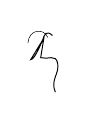
\begin{tikzpicture}[x=0.6cm,y=0.6cm]
\draw[line width=0.18pt] (0.08,1.08) .. controls (0.10,1.38) and (0.42,1.40) .. (0.50,1.20);
\draw[line width=0.35pt] (0.60,1.24) .. controls (0.48,1.35) and (0.43,1.28) .. (0.39,1.14) -- (0.14,0.73) .. controls (0.23,0.72) and (0.40,1.18) .. (0.42,1.20) -- (0.35,0.77) .. controls (0.50,0.72) and (0.67,0.86) .. (0.71,0.65) .. controls (0.75,0.42) and (0.55,0.31) .. (0.66,0.04);
\end{tikzpicture}}}

Décomposition spectrale \deleted{\unsure{de}} $|u|=\sum\ell_i\overline e_i\otimes e_i$, (les $\ell_i\geq0$)
on aura
\[
(****)\qquad\boxed{u:\sum\ell_i\deleted{\unsure{f_i}}\overline e_i\otimes f_i},
\]
où $f_i=Ue_i$, les $f_i$ forment un système orthonormal. \deleted{\illegible{3}}
\deleted{\unsure{On a de plus} $u^*=\sum\ell_i\overline f_i\otimes\unsure{e_i}$}.
Réciproquement, via une telle décomposition, on tire $|u|=\sum\ell_i\overline e_i\otimes e_i$, donc les $\ell_i$ sont les valeurs propres de $|u|$, et les $e_i$ les vecteurs propres correspondants, \unsure{on tire|les $f_i$} de ****
\[
u^*=\sum\ell_i\overline f_i\otimes e_i,
\]
donc \uuline{$|u^*|$ a les mêmes valeurs propres que $|u|$}. \unsure{\illegible{1}}
\mspage{39}

\scanpage{39}
\deleted{\unsure{Rappelons la caractérisation}}

Notations $(\lambda_i(u))$ si $u\in L_0(E)$ : c'est la suite des valeurs \inserted{\deleted{\illegible{3}}} propres de $u$, rangées par ordre de modules non \unsure{décroissants|croissants}, complétée par des $0$ si cette suite est finie.
Si la dim de $E$ est finie, \inserted{soit $n$}, \inserted{il y a lieu d'attacher \deleted{\unsure{et les}} \unsure{l'on range les} \unsure{finies} \unsure{en gardant même} \unsure{du point de vue du rang} $n+1$} \unsure{on joint} \deleted{seulement} à $\lambda_n(u)$ \unsure{les} \unsure{premiers} \unsure{termes} \unsure{nuls}.
\margin{?\unsure{!}}
De plus \deleted{$\rho_n(u)=$}, pour $u\in L_0(E,F)$,
\[
\boxed{\rho_n(u)=\lambda_n(|u|)}
\]
donc $\rho_n(u)$ est une suite décroissante de nbs positifs.

\deleted{$\unsure{\rho_n(u)}\leq\|u\|$}\qquad\deleted{$\unsure{\lambda_n(u)}$}
\[
\boxed{|\lambda_1(u)|\leq\rho_1(u)=\|u\|}\qquad
\boxed{\rho_n(u)=\rho_n(u^*)}
\]
Si $h$ est hermitien positif, on sait que
\[
\boxed{\rho_n(h)=\inf_{E_{n-1}}\deleted{\sup_{\unsure{x\in F}}\unsure{\|h_F\|}}\left(\sup_{\substack{x\in E_{n-1}\\\|x\|\leq1}}(hx,x)\right)^{\unsure{1/2}}}
\]
où \deleted{$\unsure{h_F}$} $E_{n-1}$ parcourt \deleted{\unsure{les espaces} $F:E_{\unsure{n}}$ \unsure{la forme}} les sous-espaces \unsure{vectoriels} fermés de codimension $n-1$.
\deleted{\unsure{contribution} $(hx,y)$}

On a aussi
\[
\rho_n(h^{\unsure{*|2}})^2=\rho_n(h^2)=\inf_{E_n}\sup_{\substack{x\in E_n\\\|x\|\leq1}}\|hx\|^2,
\]
\uline{d'où}
\deleted{$\rho_n(u)=\inf\sup_{x\in E_n}hx$}

\deleted{d'où $\rho_n(u)^2=\rho_n(u^*u)=\inf_{\unsure{E_n}}\sup_{x\in E_n}\|u^*ux\|$}
\[
\rho_n(h)=\inf_{E_n}\sup_{\substack{x\in E_{n-1}\\\|x\|\leq1}}\|hx\|\deleted{\unsure{{}^2}}\qquad(h\geq0)
\]
\deleted{\illegible{1}}
D'où, en prenant $h=|u|$,
\[
\boxed{\rho_n(u)=\inf_{E_n}\sup_{\substack{x\in E_{n-1}\\\|x\|\leq1}}\|ux\|}.
\]
On \deleted{\unsure{en conclut}} \inserted{conclut} aussitôt :
\[
\boxed{\begin{aligned}
\rho_n(uv)&\leq\|u\|\rho_n(v)\\
\rho_n(uv)&\leq\|v\|\rho_n(u)
\end{aligned}}
\]
Et de même : \uline{$\rho_n(h)$ est fonction croissante de l'hermitien positif $h$}.
\deleted{\uline{Corollaire} Soit $u\in L_0(E,F)$}
\deleted{\unsure{En posant} $\boxed{\unsure{\left(\sum\rho_n(u)^p\right)^{1/p}=\|u\|_p}}$}

\deleted{\unsure{Les deux théorèmes} \illegible{1}}
Les inégalités de \unsure{Ky-Fan|ky-Fan}
\[
\boxed{\begin{aligned}
\rho_{\unsure{m+n+1|m+n-1}}(AB)&\leq\rho_{m+1}(A)\rho_{n+1}(B)\\
\rho_{\unsure{m+n+1|m+n-1}}(A+B)&\unsure{<|\leq}\rho_{m+1}(A)+\rho_{n+1}(B)
\end{aligned}}
\]
\margin{?}
\mspage{40}

\scanpage{40}
\uline{II.} Caractérisation des op. de Fredholm : $u\in L^{(1)}(E,F)\Longleftrightarrow\sum\rho_i(u)<+\infty$; et alors on a
\[
\boxed{\|u\|_1=\sum\rho_i(u)}.
\]
\unsure{Corollaire 1} $u$ Fredholm $\Longleftrightarrow |u|$ Fredholm, et $\|u\|_1=\||u|\|_1=\operatorname{Tr}|u|$.

\uline{\unsure{Corollaire 2}} On a alors $|\operatorname{Tr}u|\leq\sum\rho_i(u)$.
\margin{Notation $L^{(1)}(E,F)$ et $E\widehat\otimes^{(1)}F$}
\margin{$n\leq\dim E,\ \dim F$ \uline{\unsure{Théorie de Riesz}}}

\uline{\unsure{Remarque 2}} Si $u\in L_0(E,E')$ :
\[
\boxed{\sum_1^n\rho_i(u)=\deleted{\unsure{\sum}}\sup|\operatorname{Tr}v_nu|}\qquad
\begin{gathered}
v_n\in L(E',E)\\
\|v_n\|\leq1\\
\operatorname{rang}v_n\leq n
\end{gathered}
\]
\deleted{\unsure{$v_n$ projecteur} \unsure{orthogonal}}
où le sup est atteint aux \deleted{\unsure{projections orthogonales de rang} $n$} \unsure{où} \unsure{$v_n$ est} \inserted{$v_n=p_nv_n$ ($p_n$ \unsure{projection|projecteur} \unsure{hermitien} de rang $n$)} \unsure{si} $\unsure{u}$ est \unsure{hermitien}. \deleted{dans $E$} \inserted{de dim $E\geq n$}.

\deleted{En effet on a
\[
\operatorname{Tr}p_nu=\operatorname{Tr}p_n^2u=\operatorname{Tr}p_nup_n,
\]
\unsure{soit} $w$ la restriction de $p_nup_n$ à $p_n(E)$, on a
\[
\deleted{\unsure{|\operatorname{Tr}p_nup_n|=}}\quad
|\operatorname{Tr}p_nu|=|\operatorname{Tr}w|\leq\deleted{\unsure{\dim E}}\sum_1^n\rho_i(w),
\]
or
\[
\rho_i(w)=\rho_i(p_nup_n)\leq\rho_i(up_n)\leq\rho_i(u),
\]
d'où $|\operatorname{Tr}p_nu|\leq\sum_1^n\rho_i(u)$.}

\deleted{D'où $|\operatorname{Tr}v_nu|\leq\sum_1^n\rho_i(u)$, et si $u=\sum_1^\infty\rho_i\overline e_i\otimes f_i$;}
\deleted{\unsure{Réciproquement}} \deleted{\unsure{En effet}}
\inserted{car $\rho_i(uv_n)\leq\rho_i(u)\|v_n\|=\rho_i(u)$.}
\deleted{\unsure{On peut} prouver $|\operatorname{Tr}v_nu|\leq\sum_1^n\rho_i(u)$, \unsure{il suffit de} l'inégalité}

\deleted{\unsure{Soit} $w$ un op. \inserted{de rang $\leq n$}, et $w=p_nw$, $p_n$ un projecteur de rang $n$, et $\operatorname{Tr}w=\operatorname{Tr}p_nw=\operatorname{Tr}p_n^2w=\operatorname{Tr}\figure{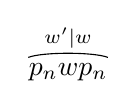
\begin{tikzpicture}[baseline=(pnwpn.base)]
\node[inner sep=0pt] (pnwpn) {$p_nwp_n$};
\draw[line width=0.4pt] ([yshift=2pt]pnwpn.north west) .. controls ([xshift=5pt,yshift=4pt]pnwpn.north west) and ([xshift=-5pt,yshift=4pt]pnwpn.north east) .. ([yshift=2pt]pnwpn.north east);
\node[anchor=south,inner sep=0pt] at ([yshift=5pt]pnwpn.north) {$\scriptstyle\inserted{\unsure{w'|w}}$};
\end{tikzpicture}}$. \unsure{On soit|On sait si} $w'$ la restriction \unsure{de} $p_nwp_n$ à $p_n(E)$, on obtient
\[
\unsure{|\operatorname{Tr}w|=}\quad|\operatorname{Tr}w'|\leq\sum_1^n\rho_i(w'),
\]
$\unsure{w'=}$
\[
\rho_i(w')=\deleted{\unsure{\rho_i(p_nwp_n)}}\deleted{\unsure{\|p_n\|}}=\rho_i(wp_n)\leq\rho_i(w),
\]
$\boxed{\rho_i(w')\leq\rho_i(w)}$, \deleted{\unsure{w sur un espace de}} \unsure{d'où l'inégalité} $\unsure{\sum\rho_i(w)}$.}

\margin{$|\operatorname{Tr}v_nu|\leq\sum_1^n\rho_i(u)$ \unsure{est une} \inserted{conséquence} \unsure{du} \uline{lemme} Si $w$ est un opérateur \unsure{\deleted{linéaire}|linéaire} de rang $\leq n$ de $E$ dans lui,
\[
|\operatorname{Tr}w|\leq\sum_1^n\rho_i(w).
\]
En effet, soit $v$ la restriction de $w$ à $w(E)$, alors on a $|\operatorname{Tr}w|=|\operatorname{Tr}v|\leq\sum_1^n\rho_i(\unsure{w|v})$ $(\unsure{\text{---}})$.
Or $v=\alpha^*w\alpha$, où $\alpha$ est l'injection \unsure{canonique} de $w(E)$ dans $E$, d'où $\rho_i(v)\leq\|\alpha^*\|\|\alpha\|\rho_i(w)\leq\rho_i(w)$, d'où $|\operatorname{Tr}w|\leq\sum_1^n\rho_i(w)$.}

Pour prouver que la borne est \inserted{atteinte} \deleted{\unsure{obtenue}}, on écrit $u=\sum_1^{\unsure{n|\infty}}\rho_i\overline e_i\otimes f_i$, et on prend
\[
v_n=\sum_{j=1}^n\overline{\unsure{f_j|f_i}}\otimes\unsure{e_j|e_i},
\]
\margin{\figure{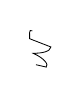
\begin{tikzpicture}[x=0.5cm,y=0.5cm]
\draw[line width=0.3pt] (0.18,1.00) .. controls (0.07,1.07) and (0.12,0.87) .. (0.11,0.80) -- (0.65,0.59) .. controls (0.63,0.47) and (0.42,0.43) .. (0.20,0.43) .. controls (0.49,0.30) and (0.60,0.14) .. (0.53,0.08) -- (0.27,0.14);
\end{tikzpicture}}}
on a \deleted{\unsure{alors}}
\[
v_nu=\sum_{\substack{ij\\j\leq n}}\rho_i\overline e_i\otimes e_j\,(f_i,f_j)
=\sum_{j\leq n}\rho_{\unsure{i|j}}\overline e_{\unsure{i|j}}\otimes\unsure{e_j|e_i},
\]
dont la trace est $\sum_1^n\rho_i$, $v_n$ est un projecteur hermitien si $u$ était supposé hermitien $(f_i=e_i)$.
\margin{(?)}
\unsure{Comme les particuliers en un corollaire, on a}

\uline{Corollaire \unsure{4|3}} Soient $u,v\in L_0(E,F)$, alors
\[
\boxed{\sum_1^n\rho_i(u+v)\leq\sum_1^n\bigl(\rho_i(u)\unsure{-|+}\rho_i(v)\bigr)}.
\]
Cas particulier $\|u+v\|_1\leq\|u\|_1+\|v\|_1$.
On peut aussi dire que $\sum_{i=1}^n\rho_i$ est une ``\uline{norme}'' sur $L_0(E,F)$.

\margin{\figure{\begin{tikzpicture}[x=0.6cm,y=0.6cm]
\draw[line width=0.3pt] (0,0.08) .. controls (0.30,-0.02) and (0.66,0.01) .. (0.79,0.26) .. controls (0.93,0.07) and (1.19,0.03) .. (1.40,0.13);
\fill (1.55,0.18) circle (0.015);
\end{tikzpicture}}}

\uline{\unsure{Dém}}
\mspage{41}

\scanpage{41}
\unsure{Introduction} de $L^p(E,F)$ et de \deleted{$\unsure{\|\ \|_p}$}
\[
\left\{\begin{aligned}
\|u\|_p&=\left(\sum\rho_i(u)^p\right)^{1/p}\\
S_p(u)&=\sum(\rho_i(u))^p
\end{aligned}\right.
\]
\unsure{Quelques} \unsure{propriétés} \illegible{2}. Cas $p=+\infty$, $p=1$.
\mspage{42}

\scanpage{42}
Dual de $L_0(E,F)$. \deleted{\unsure{Cet}} \unsure{Mettons cet espace en dualité naturelle} avec $L^{(1)}(F,E)$, \deleted{\unsure{soit}} par
\[
\boxed{(u,v)=\operatorname{Tr}vu}
\]
(les $E'\otimes F$ et $F'\otimes E$, \unsure{cela comme on sait bien})
et l'application naturelle de $L^1(F,E)$ dans $(L_0(E,F))'$ est une isométrie : si $v\in L^1(F,E)$ et est $\sum\unsure{\rho_i|\lambda_i}\overline f_i\otimes e_i$, il suffit de prendre $u=\sum_1^n\unsure{\rho_i}\overline e_i\otimes f_i$ pour trouver $(u,v)=\sum_1^n\rho_i$.
Montrons qu'il est \uline{sur}. En effet, si $\varphi$ est une forme linéaire continue sur $L_0(E,F)$, alors $\varphi(x'\otimes y)$ est une forme bilinéaire continue sur $E'\times F$, donc définit une application linéaire $F\longrightarrow E$, \unsure{soit} le $v$. On a $\varphi(u)=\operatorname{Tr}vu$, il reste à montrer que $v$ est de Fredholm, sachant $|\operatorname{Tr}vu|\leq M\|u\|$ pour $u\in E'\otimes F$.

\deleted{Considérons $\unsure{w=vv^*}\in L(E,E)$, on a \deleted{$\unsure{\operatorname{Tr}uvv^*=\operatorname{Tr}v^*uv}$} \deleted{$u\in\unsure{L(E,E)}$} \unsure{$u\in E'\otimes E$}
\[
|\operatorname{Tr}uw|=|\operatorname{Tr}uvv^*|=|\operatorname{Tr}v^*uv|\leq M\|v^*u\|;
\]
donc $w$ a la même propriété que $v$. Or \deleted{\illegible{3}} \unsure{$w$ est encore un op.} compact (donc $v$ sera compact) :}

$w=(vv^*)^{1/2}\in L(E,E)$, alors $v=Ww$, $w=Vv$, on voit aussitôt que $w\inserted{{}=Vv}$ \deleted{\unsure{est}} vérifie \unsure{la propriété} de $v$, montrons que $w$ est op. de Fredholm, donc $v\inserted{{}=Ww}$ le sera (le \unsure{précédent} : $F=E$).
Or \deleted{\illegible{1}} d'abord $w$ est cpt, \unsure{car} autrement il \unsure{existerait} un sous espace $H\subset E$ \uline{\unsure{stble}} \inserted{stable} \uline{par} \inserted{sous} $w$, où $w$ serait inversible, ce qui amène une contradiction.
\margin{\figure{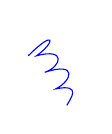
\begin{tikzpicture}[x=0.35cm,y=0.35cm]\draw[blue] (0,1.8) .. controls (1,2.8) and (1,2.3) .. (0.3,1.8) .. controls (1.4,2.1) and (1.2,1.4) .. (0.6,1.2) .. controls (1.8,1.6) and (1.6,0.9) .. (1,0.6) .. controls (2,0.8) and (1.5,0.2) .. (1.4,0);\end{tikzpicture}}}
On aura donc $w=\sum\rho_i\overline f_i\otimes e_i$, et prenant $u=\sum_1^n\overline e_i\otimes f_i$, on trouve
\[
\sum_1^n\rho_i\leq M.
\]
D'où la conclusion.
\margin{\figure{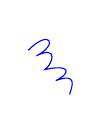
\begin{tikzpicture}[x=0.35cm,y=0.35cm]\draw[blue] (0,1.6) .. controls (0.8,2.4) and (1.1,1.8) .. (0.3,1.4) .. controls (1.1,1.8) and (0.9,1.1) .. (0.6,0.9) .. controls (1.5,1.1) and (1.6,0.8) .. (1,0.5) .. controls (1.8,0.8) and (1.6,0.3) .. (1.5,0);\end{tikzpicture}}}

--- \unsure{Méthode} \inserted{méthode} plus élémentaire : $\varphi$ est une forme linéaire continue sur $L^{\unsure{2}}(E,F)$, donc donnée par un $v\in L^2(F,E)$, qui est en particulier cpt. On achève comme tout à l'heure.
\mspage{43}

\scanpage{44}
1 \uline{Rappels} \deleted{\unsure{définitions}} et notations. Opérateurs de Fredholm

2. \uline{\unsure{Produits tensoriels hilbertiens}. \deleted{\unsure{Opérateurs Fredholm}} et de Hilbert-Schmidt}
\margin{\unsure{Traitement} \illegible{3} $\unsure{\Psi}$ est \unsure{vectoriel} \unsure{symétrique}.}

Soit $E$ un espace de \unsure{Banach} (sur le corps des réels ou complexes), désignons par $\overline E\deleted{\unsure{{}^*}}$ l'espace \deleted{\unsure{de base}} vectoriel obtenu en prenant sur $E$ la structure vectorielle \uline{ayant} la même structure additive que $E$, mais où la multiplication scalaire est donnée par $(\lambda,x)\longrightarrow\overline\lambda.x$.
\deleted{\unsure{$\overline E$ est ainsi}}
On a $\lambda\overline x=\overline{\overline\lambda x}$.
On a bien là une \deleted{\unsure{loi de groupe}} \inserted{structure d'espace} vectoriel, \deleted{et la fonction $\|x\|$ sur $\overline E$ est encore une norme}.
L'application canonique \inserted{$x\longrightarrow\overline x$} de $E$ sur $\overline E$ est antilinéaire, i.e \unsure{elle est} additive, et satisfait à :
\[
\overline{\lambda x}=\overline\lambda\,\overline x,
\]
\deleted{\unsure{c'est de plus une isométrie (au point de vue de l'application}\ \unsure{de l'espace de Banach} $\overline E$).}
Notons qu'on a aussi
\[
\overline{\overline E}=E.
\]
\margin{(1) Bien entendu, si le corps des scalaires est le corps des réels, \deleted{$\overline E=E$} $\overline E$ \unsure{possède} la même \unsure{structure} que $E$, \illegible{4}.}

\deleted{$\unsure{E=\overline E}$ \illegible{4}}
\deleted{Si $F$ est un espace vectoriel, une application antilinéaire de $E$ dans $F$ \unsure{est encore une} application linéaire de $\overline E$ dans $F$, \unsure{et de plus} \illegible{2}.}

$E,F$, \deleted{\unsure{étant}} \inserted{\unsure{deux}} espaces vectoriels, une application $(x,y)\longrightarrow u(x,y)$ \deleted{\uline{bilinéaire}} de $E\times F$ \deleted{\unsure{est dite}} dans $\mathbf C$ se dit \uline{sesquilinéaire} si elle est linéaire en $x$, et antilinéaire en $y$ ; cela signifie donc aussi bien qu'elle est une application \uline{bilinéaire} de $E\times\overline F$ dans $\mathbf C$. Ces applications correspondent donc exactement aux applications linéaires de $E\otimes\overline F$ dans $\mathbf C$.
\margin{\unsure{$L^h$}}
\margin{Notons aussi $L(E,F)=L(\overline E,\overline F)$}

\deleted{Si $E$ est un espace de Banach, on \illegible{3} de l'espace $\overline E$ \illegible{4} une norme $\|x\|$ \illegible{2}.}
\mspage{45}

\scanpage{45}
Notons que pour deux espaces vectoriels $E,F$, on a un isomorphisme canonique
\[
(2)\qquad\overline{E\otimes F}=\overline E\otimes\overline F.
\]
En effet, l'application $(\overline x,\overline y)\longrightarrow\unsure{\overline{x\otimes y}|\overline{\overline x\otimes\overline y}}$ de $\overline E\unsure{\times|\otimes}\overline F$ dans $\overline{E\otimes F}$ est manifestement bilinéaire, donc se prolonge en une application linéaire $\overline E\otimes\overline F\longrightarrow\overline{E\otimes F}$.
On vérifie alors aussitôt, au moyen des bases de $E$ et $F$ par exemple, que \unsure{c'est là} un isomorphisme du premier espace \uline{sur} le second.

\deleted{Supposons} Rappelons qu'on appelle espace \uline{préhilbertien} un espace vectoriel $E$, muni d'une forme sesquilinéaire sur $E\times E$, \deleted{\unsure{à valeurs dans C}} \inserted{dont la} valeur pour les éléments $x,y$ est notée $\langle x,y\rangle$, satisfaisant à la condition $\langle x,x\rangle\geq0$ pour tout $x$. Alors,
\deleted{\unsure{Nous obtenons ainsi une} \unsure{fonction} \illegible{3} $E\unsure{\otimes}$}
$\|x\|=\sqrt{\langle x,x\rangle}$ est une semi-norme sur $E$, et $E$ est dit un \uline{espace de Hilbert} si $E$ est séparé et complet pour cette norme.
\deleted{\illegible{5}}\deleted{\unsure{Séparé hilbertien}}
Notons \unsure{uniquement}.....

\margin{\deleted{Si à tout $y\in E$ on fait correspondre la forme linéaire $x\longrightarrow(x,y)$ sur $E$, on définit une application \deleted{\unsure{linéaire}} \inserted{\unsure{antilinéaire}} de $E$ sur le dual $E'$, conservant la norme. Par suite, on a un isomorphisme \uline{\unsure{canonique}} \unsure{d'espaces} \illegible{1}
\[
(3)\qquad E'=\overline E\qquad(E\text{ Hilbert}).
\]}}

\unsure{Soient maintenant} $E$ et $F$ deux espaces \deleted{préhilbertiens} \inserted{de Hilbert}, on \unsure{mettra} sur $E\otimes F$ une structure \deleted{préhilbertienne} \inserted{d'espace préhilbertien séparé} \inserted{canonique}.
Pour ceci, on doit définir une forme linéaire sur $(E\otimes F)\otimes\overline{E\otimes F}$ ; \deleted{\unsure{donc}} en vertu de (2), \deleted{\unsure{une forme}} cet espace est isomorphe canoniquement à $(E\otimes\overline E)\otimes(F\otimes\overline F)$ ; il faut donc définir une forme linéaire sur ce dernier, \unsure{on en connaît une}
\margin{Introduire sur $E\otimes F\subset L(\overline E,F)$ la forme \uline{$\operatorname{Tr}(v^*u)$} directement}
\mspage{46}

\scanpage{46}
Notons que pour deux espaces vectoriels $E,F$, on a un isomorphisme canonique
\[
(2)\qquad\overline{E\otimes F}=\overline E\otimes\overline F.
\]
En effet, l'application $(\overline x,\overline y)\longrightarrow\unsure{\overline{x\otimes y}|\overline{\overline x\otimes\overline y}}$ de $\overline E\unsure{\times|\otimes}\overline F$ dans $\overline{E\otimes F}$ est manifestement bilinéaire, donc se prolonge en une application linéaire $\overline E\otimes\overline F\longrightarrow\overline{E\otimes F}$
\margin{\deleted{la forme linéaire \par \unsure{application} \deleted{\unsure{linéaire}} antilinéaire. \par \unsure{norme}. Par suite, on a}}

Notons maintenant que si $E$ est un espace préhilbertien, alors la fonction $\overline x,\overline y\longrightarrow\unsure{(y,x)}$ sur $\overline E\times\overline E$ est une forme sesquilinéaire ; qu'on notera $(\overline x,\overline y)$ ; qui \deleted{\unsure{fait} \illegible{2} $\overline E$ \illegible{3}} est \deleted{\unsure{définie}} \inserted{\unsure{encore}} positive, car $(\overline x,\overline x)=(x,x)$.
Ceci permet de considérer $\overline E$ comme un espace préhilbertien.
\[
(3)\qquad(\overline x,\overline y)=(y,x)
\]
Comme on a $\|x\|=\|\overline x\|$, la norme de $\overline E$ coïncide avec celle de $E$. Si donc $E$ est séparé, $\overline E$ l'est, et \uline{si $E$ est un espace de Hilbert, $\overline E$ est aussi un espace de Hilbert}.
Dans ce dernier cas, on sait que l'application qui à tout $y\in E$ fait correspondre la forme $x\longrightarrow(x,y)$ sur $E$, est une \deleted{\unsure{isométrie}} \inserted{\unsure{appl. bijective}} \uline{antilinéaire} de $E$ \uline{sur} le dual $E'$, conservant la norme, par suite, on a \deleted{\unsure{de façon}} \inserted{ainsi} un isomorphisme canonique d'espaces normés :
\[
(4)\qquad E'=\overline E\qquad(E,\text{ espace de Hilbert})
\]
Cet isomorphisme permet de considérer $E'$ comme \deleted{\unsure{muni de la} \illegible{2}} \deleted{\unsure{forme de} \illegible{2}} un espace de Hilbert.
\mspage{47}

\scanpage{48}
forme $4$ fois linéaire sur $E\times\overline E\times F\times\overline F$.
\deleted{\unsure{Dans ceci}} \inserted{Ceci montre} qu'on peut considérer dans $E\otimes F$ \deleted{\unsure{la structure préhilbertienne}} une forme sesquilinéaire $(u,v)$ définie par \deleted{\unsure{une formule}} :
\[
(5)\qquad\boxed{(x_1\otimes y_1,x_2\otimes y_2)=(x_1\deleted{\otimes},x_2)(y_1\deleted{\otimes},y_2)}
\]
(car le deuxième membre de (\unsure{3|5}) est bien linéaire en $x_1\in E$, $x_2\in\overline E$, $y_1\in F$, $y_2\in\overline F$).
\deleted{Montrons que} \inserted{Montrons} qu'on a bien là une forme \unsure{définie positive}.
\deleted{cette forme est une forme définie positive, i.e que $(u,u)\geq0$ et $(u,u)=0\Longleftrightarrow u=0$.
\deleted{En effet} Soit $(e_i)_{i\in I}$ une base orthonormale dans $E$, $(f_j)_{j\in J}$ une base orthonormale dans $F$, alors $(e_i\otimes f_j)_{(ij)\in I\times J}$}

\deleted{En effet, si $\unsure{u}\in E\otimes F$, alors $\unsure{u}$ \unsure{est dans}}
\deleted{$\unsure{u}\in E_0\otimes F_0$, où} \inserted{Donnons-nous} $E_0$ et $F_0$ \deleted{sont} deux sous-espaces de dim finie de $E$ et $F$, \deleted{Prenons alors} \inserted{et prenons} une base orthonormale \inserted{$(e_i)$} dans $E_0$, une autre $(f_j)$ dans $F_0$,
\deleted{\unsure{on aura} $u=\sum$}
alors $(e_i\otimes f_j)$ est une base de l'espace vectoriel, et on sait par (\unsure{5}) que
\[
(6)\qquad(e_i\otimes f_j,e_{i'}\otimes f_{j'})=\delta_{(ij),(i'j')}\qquad\text{(indice de Kronecker)}
\]
ce qui prouve que $(u,v)$ induit sur $E_0\otimes F_0$ une forme \uline{définie positive}.
Comme $E\otimes F$ est réunion des espaces $E_0\otimes F_0$, cela prouve que $(u,v)$ est \uline{définie} positive.

\uline{Définition} Soient $E,F$ deux espaces de Hilbert. On appelle produit tensoriel hilbertien de $E$ et $F$, et on note $E\overset{(2)}{\otimes}F$, le complété de l'espace \deleted{$\unsure{E}$} $E\otimes F$ préhilbertien
\mspage{49}

\scanpage{49}
séparé $E\otimes F$, \deleted{\unsure{dont}} \inserted{\unsure{où}} le produit scalaire est défini par (5).
La norme d'un élément \deleted{\illegible{2}} $u\in E\overset{(2)}\otimes F$ est notée $\|u\|_2$.
$E\overset{(2)}\otimes F$ est donc un espace de Hilbert.

\uline{Prop. 1} Soient $E$ et $F$ deux espaces de Hilbert. \deleted{\unsure{$x\in E$, $y\in F$,}}
\deleted{$\|x\otimes y\|_2=\|x\|\|y\|\unsure{{}^2}$}
Soit $(e_i)_{i\in I}$ une base orthonormale dans $E$, $(f_j)_{j\in J}$ une base orthonormale dans $F$, alors $(e_i\otimes f_j)_{(ij)\in I\times J}$ est une base orthonormale dans $E\overset{(2)}\otimes F$.

En effet, d'après (\unsure{4|6}) le système $(e_i\otimes f_j)$ est orthonormal, \deleted{de plus les \unsure{combinaisons finies sont denses dans} $E\overset{(2)}\otimes F$.}
\deleted{En effet, \illegible{2}} \unsure{montrons} que l'espace vectoriel qu'il engendre est dense dans $E\overset{(2)}\otimes F$.
\deleted{Pour ceci}, si $E_0$ (resp. $F_0$) \deleted{est} \inserted{désigne} l'espace engendré par les $e_i$ (resp. les $f_j$) \deleted{\unsure{et les combinaisons finies}} \deleted{\unsure{par suite}}
$E_0$ est dense dans $E$, $F_0$ dense dans $F$, donc $E_0\otimes F_0$ dense dans $E\otimes F$, donc aussi dans $E\overset{(2)}\otimes F$.

Notons aussi la formule
\[
(7)\qquad\boxed{\|x\otimes y\|_2=\|x\|\|y\|}
\]
\unsure{résulte} en effet \deleted{de} \deleted{qui résulte aussitôt de}
\[
(x\otimes y,x\otimes y)=(x,x)(y,y).
\]
\deleted{\unsure{le cas de forme} \illegible{3}}
Notons aussi que l'isomorphisme \inserted{canonique} $\overline{E\otimes F}=\overline E\otimes\overline F$ (formule (2)) conserve évidemment les structures préhilbertiennes, d'où un isomorphisme canonique
\[
(8)\qquad\overline{E\overset{(2)}\otimes F}=\overline E\overset{(2)}\otimes\overline F.
\]
\mspage{50}

\scanpage{50}
\mspage{51}

\deleted{L'exemple le plus important de produit tensoriel hilbertien
est \unsure{donné|fourni} par le

\uline{\unsure{Th|Prop}} Soit $E$ un espace de Hilbert,
\deleted{soit $\mu$ une mesure
sur un \illegible{2}}
positive sur un espace loc\textsuperscript{t} compact $M$, considérons,
l'espace de Hilbert $L^2(\mu)$, et l'espace de Hilbert}

\uline{Exemple} Soit $M$ un espace loc\textsuperscript{t} cpt muni d'une
mesure positive $\mu$, considérons l'espace de Hilbert
$L^2(\mu)$ (où $(\varphi,\psi)=\int\varphi\overline\psi\,d\mu$).
Pour tout espace de Banach $E$, $L^2_E(\mu)$ désigne l'espace des
fonctions sur $M$, à valeurs dans $E$, de \unsure{puissance deuxième}
intégrables, muni de la norme
\[
(9)\qquad
\|f\|_2=\left(\int \deleted{\unsure{f(t)}}\|f(t)\|_E^2\,d\mu(t)\right)^{1/2}
\]
qui en fait un espace de Banach $(\qquad)$. Si
$E$ est un espace de Hilbert, la norme $(9)$ peut
aussi être définie par un produit scalaire
\[
(10)\qquad (f,g)=\int\langle f(t),\overline g(t)\rangle\,d\mu(t)
\]
donc $L^2_E(\mu)$ est alors un espace de Hilbert.

On a une application bilinéaire naturelle
$(\varphi,a)\longrightarrow\varphi.a$ de $L^2\deleted{\unsure{(\mu)}}\times E$ dans $L^2_E$,
d'où une application linéaire \inserted{$u\to\widetilde u$}
$L^2\otimes E\longrightarrow L^2_E$, dont
l'image est d'ailleurs dense dans $L^2_E$. \deleted{\unsure{Il en}}
\deleted{\unsure{qui|par}} C'est un isomorphisme pour les structures
préhilbertiennes, car \inserted{on a évidemment}
$(\varphi.a,\psi.b)=(\varphi,\psi)(a,b)$,
i.e
\[
(\widetilde{\varphi\otimes a},\widetilde{\psi\otimes b})
=(\varphi\otimes a,\psi\otimes b),
\]
d'où \unsure{linéairement|linéarité} $(\widetilde u,\widetilde v)=(u,v)$
pour tous $u,v\in L^2\otimes E$.
